\chapter{SİSTEM MİMARİSİ, MODEL VE METODOLOJİ}
\label{chap:sistem}
% T-tipi faz kolu için ortak vektör çizim tabanı.
% Argümanlar: Q1, Q2, Q3, Q4 çizgi renkleri ve ek TikZ yolu.
\newcommand{\ttypevector}[5]{%
\begin{tikzpicture}[
  x=0.76cm,y=0.56cm,
  terminal/.style={circle,fill=black,inner sep=1.25pt},
  sw/.style={rounded corners=1pt,minimum width=7mm,minimum height=8mm,fill=white,font=\scriptsize},
  bus/.style={line width=0.8pt},
  current/.style={-{Latex[length=2mm]},red!80!black,line width=1.7pt},
  activepath/.style={blue!70!black,line width=2.0pt}
]
  % Bölünmüş DA bara ve kapasitörler
  \draw[bus] (0,5) -- (4,5);
  \draw[bus] (0,-1) -- (4,-1);
  \draw[bus] (0,5) -- (0,3.65);
  \draw[bus] (-0.32,3.65) -- (0.32,3.65);
  \draw[bus] (-0.32,3.35) -- (0.32,3.35);
  \draw[bus] (0,3.35) -- (0,2);
  \draw[bus] (0,2) -- (0,0.65);
  \draw[bus] (-0.32,0.65) -- (0.32,0.65);
  \draw[bus] (-0.32,0.35) -- (0.32,0.35);
  \draw[bus] (0,0.35) -- (0,-1);
  \node[font=\scriptsize,left] at (0,5) {$+V_{\mathrm{dc}}/2$};
  \node[font=\scriptsize,left] at (0,2) {$N$};
  \node[font=\scriptsize,left] at (0,-1) {$-V_{\mathrm{dc}}/2$};
  \node[font=\scriptsize,left] at (-0.38,3.5) {$C_A$};
  \node[font=\scriptsize,left] at (-0.38,0.5) {$C_B$};

  % Ana anahtarlar ve çift yönlü nötr kol
  \node[sw,draw=#1,line width=1.25pt] (q1) at (4,3.65) {$Q_1$};
  \node[sw,draw=#2,line width=1.25pt] (q2) at (4,0.35) {$Q_2$};
  \node[sw,draw=#3,line width=1.25pt] (q3) at (1.55,2) {$Q_3$};
  \node[sw,draw=#4,line width=1.25pt] (q4) at (2.75,2) {$Q_4$};
  \draw[bus] (4,5) -- (q1.north);
  \draw[bus] (q1.south) -- (4,2);
  \draw[bus] (4,2) -- (q2.north);
  \draw[bus] (q2.south) -- (4,-1);
  \draw[bus] (0,2) -- (q3.west);
  \draw[bus] (q3.east) -- (q4.west);
  \draw[bus] (q4.east) -- (5.15,2);
  \node[terminal] at (0,2) {};
  \node[terminal] (out) at (4,2) {};
  \draw[-{Latex[length=1.8mm]},thick] (out) -- (5.15,2);
  \node[font=\scriptsize,right] at (5.15,2) {$v_{xN},\ i_x$};
  #5
\end{tikzpicture}%
}

% Faz başına tam T-tipi güç devresi: bölünmüş DA bara, dört IGBT ve LCL filtre.
% Eski tezde C olarak gösterilen filtre kapasitörü, modelle tutarlılık için C_f olarak adlandırılmıştır.
\newcommand{\ttypefulltopology}{%
\begin{tikzpicture}[
  x=0.88cm,y=0.68cm,
  wire/.style={line width=0.9pt},
  coilpath/.style={decorate,decoration={coil,aspect=0.48,segment length=2.8mm,amplitude=1.8mm}},
  igbt/.style={circle,draw,line width=0.9pt,minimum size=10mm,inner sep=0pt,fill=white},
  terminal/.style={circle,fill=black,inner sep=1.35pt},
  label/.style={font=\scriptsize,align=center}
]
  % Bölünmüş DA bara ve orta nokta
  \draw[wire] (0,5) -- (5.3,5);
  \draw[wire] (0,-1) -- (5.3,-1);
  \draw[wire] (0,5) -- (0,3.65);
  \draw[wire] (-0.38,3.65) -- (0.38,3.65);
  \draw[wire] (-0.38,3.35) -- (0.38,3.35);
  \draw[wire] (0,3.35) -- (0,2);
  \draw[wire] (0,2) -- (0,0.65);
  \draw[wire] (-0.38,0.65) -- (0.38,0.65);
  \draw[wire] (-0.38,0.35) -- (0.38,0.35);
  \draw[wire] (0,0.35) -- (0,-1);
  \node[label,left] at (0,5) {$\mathrm{DC}^{+}$};
  \node[label,left] at (0,2) {$N$};
  \node[label,left] at (0,-1) {$\mathrm{DC}^{-}$};
  \node[label,left=1mm] at (-0.38,3.50) {$C_A$};
  \node[label,left=1mm] at (-0.38,0.50) {$C_B$};
  \node[terminal] at (0,2) {};

  % Ana faz kolu IGBT'leri. D_1 ve D_2 antiparalel diyotları belirtir.
  \node[igbt] (q1) at (5.3,3.65) {};
  \draw[wire] ($(q1.center)+(0,-0.30)$) -- ($(q1.center)+(0,0.30)$);
  \draw[wire] ($(q1.center)+(-0.30,-0.18)$) -- ($(q1.center)+(-0.12,-0.18)$);
  \draw[wire] ($(q1.center)+(-0.30,-0.18)$) -- ($(q1.center)+(-0.30,0.18)$);
  \node[label,right=1.5mm] at (q1.east) {$Q_1$\\IGBT+$D_1$};
  \node[igbt] (q2) at (5.3,0.35) {};
  \draw[wire] ($(q2.center)+(0,-0.30)$) -- ($(q2.center)+(0,0.30)$);
  \draw[wire] ($(q2.center)+(-0.30,-0.18)$) -- ($(q2.center)+(-0.12,-0.18)$);
  \draw[wire] ($(q2.center)+(-0.30,-0.18)$) -- ($(q2.center)+(-0.30,0.18)$);
  \node[label,right=1.5mm] at (q2.east) {$Q_2$\\IGBT+$D_2$};
  \draw[wire] (5.3,5) -- (q1.north);
  \draw[wire] (q1.south) -- (5.3,2);
  \draw[wire] (5.3,2) -- (q2.north);
  \draw[wire] (q2.south) -- (5.3,-1);
  \node[terminal] (pole) at (5.3,2) {};

  % Orta noktayı faz kutbuna bağlayan ters seri IGBT çifti
  \node[igbt] (q3) at (2.05,2) {};
  \draw[wire] ($(q3.center)+(-0.30,0)$) -- ($(q3.center)+(0.30,0)$);
  \draw[wire] ($(q3.center)+(-0.18,-0.30)$) -- ($(q3.center)+(-0.18,-0.12)$);
  \node[label,above=1.2mm] at (q3.north) {$Q_3$ (IGBT+$D_3$)};
  \node[igbt] (q4) at (3.55,2) {};
  \draw[wire] ($(q4.center)+(-0.30,0)$) -- ($(q4.center)+(0.30,0)$);
  \draw[wire] ($(q4.center)+(0.18,-0.30)$) -- ($(q4.center)+(0.18,-0.12)$);
  \node[label,below=1.2mm] at (q4.south) {$Q_4$ (IGBT+$D_4$)};
  \draw[wire] (0,2) -- (q3.west);
  \draw[wire] (q3.east) -- (q4.west);
  \draw[wire] (q4.east) -- (pole);

  % Faz başına LCL filtre ve şebeke/yük terminali
  \coordinate (l1a) at (6.35,2);
  \coordinate (l1b) at (7.45,2);
  \coordinate (cnode) at (8.15,2);
  \coordinate (l2a) at (8.85,2);
  \coordinate (l2b) at (9.95,2);
  \draw[wire] (pole) -- (l1a);
  \draw[coilpath,line width=0.9pt] (l1a) -- (l1b);
  \draw[wire] (l1b) -- (cnode) -- (l2a);
  \draw[coilpath,line width=0.9pt] (l2a) -- (l2b);
  \draw[wire,-{Latex[length=1.8mm]}] (l2b) -- (11.1,2);
  \node[label,above=1.5mm] at ($(l1a)!0.5!(l1b)$) {$L_1$};
  \node[label,above=1.5mm] at ($(l2a)!0.5!(l2b)$) {$L_2$};
  \node[label,right] at (11.1,2) {$v_g,\ i_2$};
  \node[terminal] at (cnode) {};
  \draw[wire] (cnode) -- (8.15,1.25);
  \draw[wire] (7.78,1.25) -- (8.52,1.25);
  \draw[wire] (7.78,0.95) -- (8.52,0.95);
  \draw[wire] (8.15,0.95) -- (8.15,-1.45) -- (-0.85,-1.45);
  \draw[wire] (-0.85,-1.45) -- (-0.85,2) -- (0,2);
  \node[label,right=1mm] at (8.52,1.10) {$C_f$ (eski $C$)};
  \draw[-{Latex[length=1.8mm]},red!80!black,line width=1.1pt] (6.0,2.30) -- (7.0,2.30);
  \node[label,above] at (6.5,2.30) {$i_1$};
\end{tikzpicture}%
}

% Senkron-buck eşdeğeri: üst ray, alt ray, üst ve alt anahtar etiketleri.
\newcommand{\syncbuckvector}[4]{%
\begin{tikzpicture}[
  x=0.82cm,y=0.65cm,
  sw/.style={draw,rounded corners=1pt,minimum width=8mm,minimum height=8mm,fill=white,font=\scriptsize},
  coilpath/.style={decorate,decoration={coil,aspect=0.48,segment length=2.7mm,amplitude=1.8mm}},
  current/.style={-{Latex[length=2mm]},red!80!black,line width=1.4pt}
]
  \draw[line width=0.8pt] (0,3.2) -- (1.8,3.2);
  \draw[line width=0.8pt] (0,0) -- (1.8,0);
  \node[font=\scriptsize,left] at (0,3.2) {#1};
  \node[font=\scriptsize,left] at (0,0) {#2};
  \node[sw,draw=green!55!black,line width=1.2pt] (qh) at (1.8,2.45) {#3};
  \node[sw,draw=gray!65,line width=1.2pt] (ql) at (1.8,0.75) {#4};
  \draw[line width=0.8pt] (1.8,3.2) -- (qh.north);
  \draw[line width=0.8pt] (qh.south) -- (1.8,1.6);
  \draw[line width=0.8pt] (1.8,1.6) -- (ql.north);
  \draw[line width=0.8pt] (ql.south) -- (1.8,0);
  \fill (1.8,1.6) circle (1.5pt);
  \coordinate (l1a) at (2.45,1.6);
  \coordinate (l1b) at (3.35,1.6);
  \coordinate (cnode) at (3.88,1.6);
  \coordinate (l2a) at (4.30,1.6);
  \coordinate (l2b) at (5.20,1.6);
  \draw[line width=0.8pt] (1.8,1.6) -- (l1a);
  \draw[coilpath,line width=0.9pt] (l1a) -- (l1b);
  \draw[line width=0.8pt] (l1b) -- (cnode) -- (l2a);
  \draw[coilpath,line width=0.9pt] (l2a) -- (l2b);
  \draw[current] (l2b) -- (6.0,1.6);
  \node[font=\scriptsize,above=2mm] at ($(l1a)!0.5!(l1b)$) {$L_1$};
  \node[font=\scriptsize,above=2mm] at ($(l2a)!0.5!(l2b)$) {$L_2$};
  \node[font=\scriptsize,right] at (6.0,1.6) {$v_g,\ i_L$};
  \fill (cnode) circle (1.3pt);
  \draw[line width=0.8pt] (cnode) -- (3.88,1.0);
  \draw[line width=0.8pt] (3.55,1.0) -- (4.21,1.0);
  \draw[line width=0.8pt] (3.55,0.75) -- (4.21,0.75);
  \draw[line width=0.8pt] (3.88,0.75) -- (3.88,0.2);
  \draw[line width=0.8pt] (3.58,0.2) -- (4.18,0.2);
  \draw[line width=0.8pt] (3.68,0.05) -- (4.08,0.05);
  \node[font=\scriptsize,right] at (4.18,0.88) {$C_f$};
  \draw[blue!70!black,line width=1.8pt] (0.5,3.2) -- (qh.north);
  \draw[blue!70!black,line width=1.8pt] (qh.south) -- (1.8,1.6) -- (l1a);
\end{tikzpicture}%
}


Literatür incelemesi, T-tipi dönüştürücünün yüksek verim ve güç yoğunluğu bakımından güçlü bir seçenek olduğunu; hafif yükteki ters akım, nötr kol kullanımı ve şebeke akımı harmoniklerinin ise aynı sistem sınırı içinde ele alınması gerektiğini göstermiştir. Tezde incelenen yapı, bölünmüş doğru akım (DA) bara, üç fazlı dört telli T-tipi güç katı, LCL çıkış filtresi, şebeke bağlantısı, ölçüm zinciri ve sayısal denetim biriminden oluşmaktadır. Bölümün amacı önerilen yöntemlerin uygulanacağı fiziksel sistemi tanımlamak, anahtarlama durumlarını ortak bir gösterim altında toplamak ve sonraki analizlerin dayanacağı matematiksel modeli kurmaktır.

Eski tezdeki T-tipi çalışma açıklamaları ile deney düzeneğine dağılmış teknik bilgiler yeniden düzenlenmiş; topolojiye ilişkin iddialar çok seviyeli dönüştürücü ve hafif yük literatürüyle sınanmıştır \citep{Mohan2003,Holmes2003,Schweizer2013,Wang2020,Chen2010}. Model, ideal anahtarlama durumlarını açıklayan devre düzeyi ile LCL filtre ve denetim çevrimini açıklayan ortalama değer düzeyini birbirinden ayırmaktadır. Yarı iletken gerilim düşümleri, ölü zaman, örnekleme gecikmesi ve doygunluk gibi ideal olmayan etkiler sonraki bölümlerde ayrıca devreye alınacaktır.

\section{Sistemin Genel Mimarisi ve İnceleme Sınırı}

Şekil~\ref{fig:genel-sistem-mimarisi}, enerji, ölçüm ve denetim yollarını aynı çerçevede göstermektedir. Deşarj yönünde batarya veya ayarlanabilir DA kaynak tarafından sağlanan enerji, bölünmüş DA bara üzerinden T-tipi güç katına aktarılmakta; anahtarlanan faz gerilimleri LCL filtre aracılığıyla şebeke akımına dönüştürülmektedir. Akım ve gerilim ölçümleri sayısal denetim birimine taşınmakta, üretilen modülasyon komutları kapı sürücüleri üzerinden güç katına uygulanmaktadır. Sin\textsuperscript{3} tabanlı şekillendirme yolu, akım denetleyicisinin yerine geçen bağımsız bir kontrolcü olarak değil, nötr anahtar susturma yönteminin düşük güçte oluşturduğu üçüncü harmonik bileşene karşı modülasyon girişine eklenen ikincil bir kompanzasyon terimi olarak konumlandırılmıştır.

\begin{figure}[H]
  \centering
  \resizebox{0.98\textwidth}{!}{%
  \begin{tikzpicture}[
    node distance=8mm and 8mm,
    block/.style={draw, rounded corners=1.5pt, align=center, minimum height=11mm, minimum width=24mm, fill=blue!5},
    ctrl/.style={draw, rounded corners=1.5pt, align=center, minimum height=10mm, minimum width=25mm, fill=orange!10},
    meas/.style={draw, rounded corners=1.5pt, align=center, minimum height=9mm, minimum width=24mm, fill=gray!10},
    flow/.style={-{Latex[length=2mm]}, thick},
    sig/.style={-{Latex[length=2mm]}, thick, dashed}
  ]
    \node[block] (bat) {Batarya /\\DA kaynak};
    \node[block, right=of bat] (dc) {Bölünmüş\\DA bara};
    \node[block, right=of dc] (inv) {Üç fazlı\\T-tipi güç katı};
    \node[block, right=of inv] (lcl) {LCL\\filtre};
    \node[block, right=of lcl] (grid) {Şebeke /\\ortak bağlantı};
    \draw[flow] (bat) -- node[above, font=\scriptsize]{enerji} (dc);
    \draw[flow] (dc) -- (inv);
    \draw[flow] (inv) -- (lcl);
    \draw[flow] (lcl) -- (grid);

    \node[meas, below=15mm of lcl] (meas) {Gerilim ve akım\\ölçümleri};
    \node[ctrl, left=of meas] (pwm) {PWM ve kapı\\sinyalleri};
    \node[ctrl, left=of pwm] (control) {Akım denetimi ve\\sınırlandırıcılar};
    \node[ctrl, below=of control] (sin3) {Sin\textsuperscript{3}\\kompanzasyonu};
    \draw[sig] (grid.south) |- (meas.east);
    \draw[sig] (lcl.south) -- (meas.north);
    \draw[sig] (meas) -- (control);
    \draw[sig] (control) -- (pwm);
    \draw[sig] (sin3) -- (control);
    \draw[sig] (pwm.north) |- (inv.south);
  \end{tikzpicture}%
  }
  \caption{\juriistegietiketi\ Genel sistem mimarisi.}
  \label{fig:genel-sistem-mimarisi}
\end{figure}

\begin{center}
\juriistegietiketi\ \small Genel blok diyagram; güç yolu, geri besleme yolu ve Sin\textsuperscript{3} kompanzasyonunun ikincil konumunu aynı şekil üzerinde ayırmaktadır.
\end{center}

İnceleme sınırı üç katman üzerinden kurulmuştur. Fiziksel katman yarı iletkenleri, bölünmüş DA barayı, filtreyi ve şebeke bağlantısını; denetim katmanı ölçüm, akım regülasyonu, modülasyon ve kapı sinyali üretimini; doğrulama katmanı ise benzetim ile deneyde ortak kullanılacak çalışma noktalarını ve performans ölçütlerini kapsamaktadır. GT-tipi yeniden yapılandırma, aynı yarı iletkenlerin şarj ve deşarj kiplerinde farklı görevlerde kullanılmasına dayandığından ayrıntılı işlev paylaşımı ilgili mimari bölümünde ele alınacaktır. Mevcut bölüm, deşarj yönündeki T-tipi evirici davranışını ve önerilen düşük güç yöntemlerinin dayandığı modeli sabitlemektedir.

Tek bir modelin bütün iddiaları aynı doğrulukla desteklediği varsayılmamıştır. Tablo~\ref{tab:model-katmanlari}, bölümde kullanılan model katmanlarını, her katmanın kapsadığı etkileri ve hangi iddiayı sınayacağını ayırmaktadır. Ayrım, ortalama değerli denetim modelinden elde edilen kararlılık sonucunun anahtarlama kaybı veya deneysel verim kanıtı gibi sunulmasını önlemektedir.

\begin{table}[htbp]
  \centering
  \caption{\juriistegietiketi\ Model ve doğrulama katmanlarının amaç ve kanıt sınırları.}
  \label{tab:model-katmanlari}
  \small
  \begin{tabularx}{\textwidth}{p{0.21\textwidth} p{0.27\textwidth} X X}
    \toprule
    Katman & Temel içerik & Sınanacak konu & Tek başına kanıtlamadığı konu \\
    \midrule
    İdeal anahtarlama durumu & $P$--$O$--$N$ seviyeleri ve akım yönü & Geçerli kapı durumu, gerilim seviyesi ve iletim yolu & Ölü zaman, kayıp ve THD \\
    Ortalama LCL/denetim modeli & $L_1$--$C_f$--$L_2$, gecikme ve $C_i(s)$ & Akım izleme, kutuplar ve kararlılık marjı & Yarı iletken geçiş kaybı \\
    Anahtarlamalı benzetim & Gerçek PWM, kapı mantığı ve ideal olmayan elemanlar & Ters akım, harmonikler, anahtarlama sayısı ve geçici rejim & Donanım sıcaklığı ve ölçüm belirsizliği \\
    Deneysel sistem & Güç katı, sensör, sürücü, ADC ve gerçek zamanlı kod & Verim, THD, koruma ve uygulanabilirlik & Test edilmeyen çalışma bölgesine genelleme \\
    \bottomrule
  \end{tabularx}
\end{table}

\section{T-Tipi Faz Kolu ve Anahtarlama Durumları}

Üç seviyeli T-tipi faz kolunda üst ana anahtar $Q_1$, alt ana anahtar $Q_2$ ve DA bara orta noktasını faz çıkışına bağlayan çift yönlü nötr kol anahtarları $Q_3$ ile $Q_4$ olarak adlandırılmıştır. Önceki tezin Şekil~3.1'inde verilen tek faz kolu şeması, topoloji literatürüyle birlikte Şekil~\ref{fig:t-tipi-faz-kolu} üzerinde Bölüm~2'ye aktarılmıştır; aynı devre burada gereksiz tekrar oluşturmaması için yeniden basılmamıştır. Bölünmüş bara geriliminin toplamı $V_{\mathrm{dc}}$ kabul edildiğinde ideal faz-kutup gerilimi $+V_{\mathrm{dc}}/2$, $0$ ve $-V_{\mathrm{dc}}/2$ seviyelerinden birini alır. Nötr kolun eklediği sıfır seviyesi, iki seviyeli yapıya göre daha küçük gerilim basamakları oluşturur; bunun karşılığında komütasyon düzeni ile nötr nokta akımının ayrıca yönetilmesi gerekir \citep{Schweizer2013,Wang2020}.

Sonradan sağlanan tam topoloji Şekil~\ref{fig:gelen-tam-topoloji} üzerinde sistem sınırını kesinleştirmiştir. Şemanın solunda dört iletkenli giriş, ortak-mod endüktansları ve şönt kapasitörlerden oluşan giriş/EMI ağı; ortasında ortak DA bağlantısına bağlanan üç tekrarlı T-tipi faz hücresi; her hücrede dış kol anahtar modülü, çift yönlü nötr kol, doğrultucu diyotlar, yerel kapasitörler, akım algılama elemanı ve röle; alt bölümünde ise fazlara ilişkin gerilim algılama transformatörleri görülmektedir. Şemadaki $L1$, $L2$ ve $L3$ etiketleri LCL filtrenin ardışık $L_1$--$L_2$ elemanlarını değil, sırasıyla A, B ve C fazlarına ait üç eş \SI{600}{\micro\henry} bobini göstermektedir. Bu ayrım, $L2=\SI{600}{\micro\henry}$ etiketinin filtredeki ikinci bobin sanılmasından kaynaklanan görünür çelişkiyi gidermektedir. Tezde bütün topoloji üç amaçla kullanılmaktadır: sistem ve ölçüm sınırını belirlemek, üç fazın aynı faz-başına modelin tekrarı olduğunu göstermek ve yarı iletken/parazit parametrelerini gerçek devre elemanlarıyla eşlemek. Anahtarlama denklemleri ve akım yolu çizimleri okunabilirlik için Şekil~\ref{fig:t-tipi-akim-yollari}'ndaki tek faz eşdeğerine indirgenmiştir; bu indirgeme giriş filtresinin, diğer iki fazın veya ölçüm/koruma elemanlarının fiziksel sistemde bulunmadığı anlamına gelmez.

\begin{figure}[htbp]
  \centering
  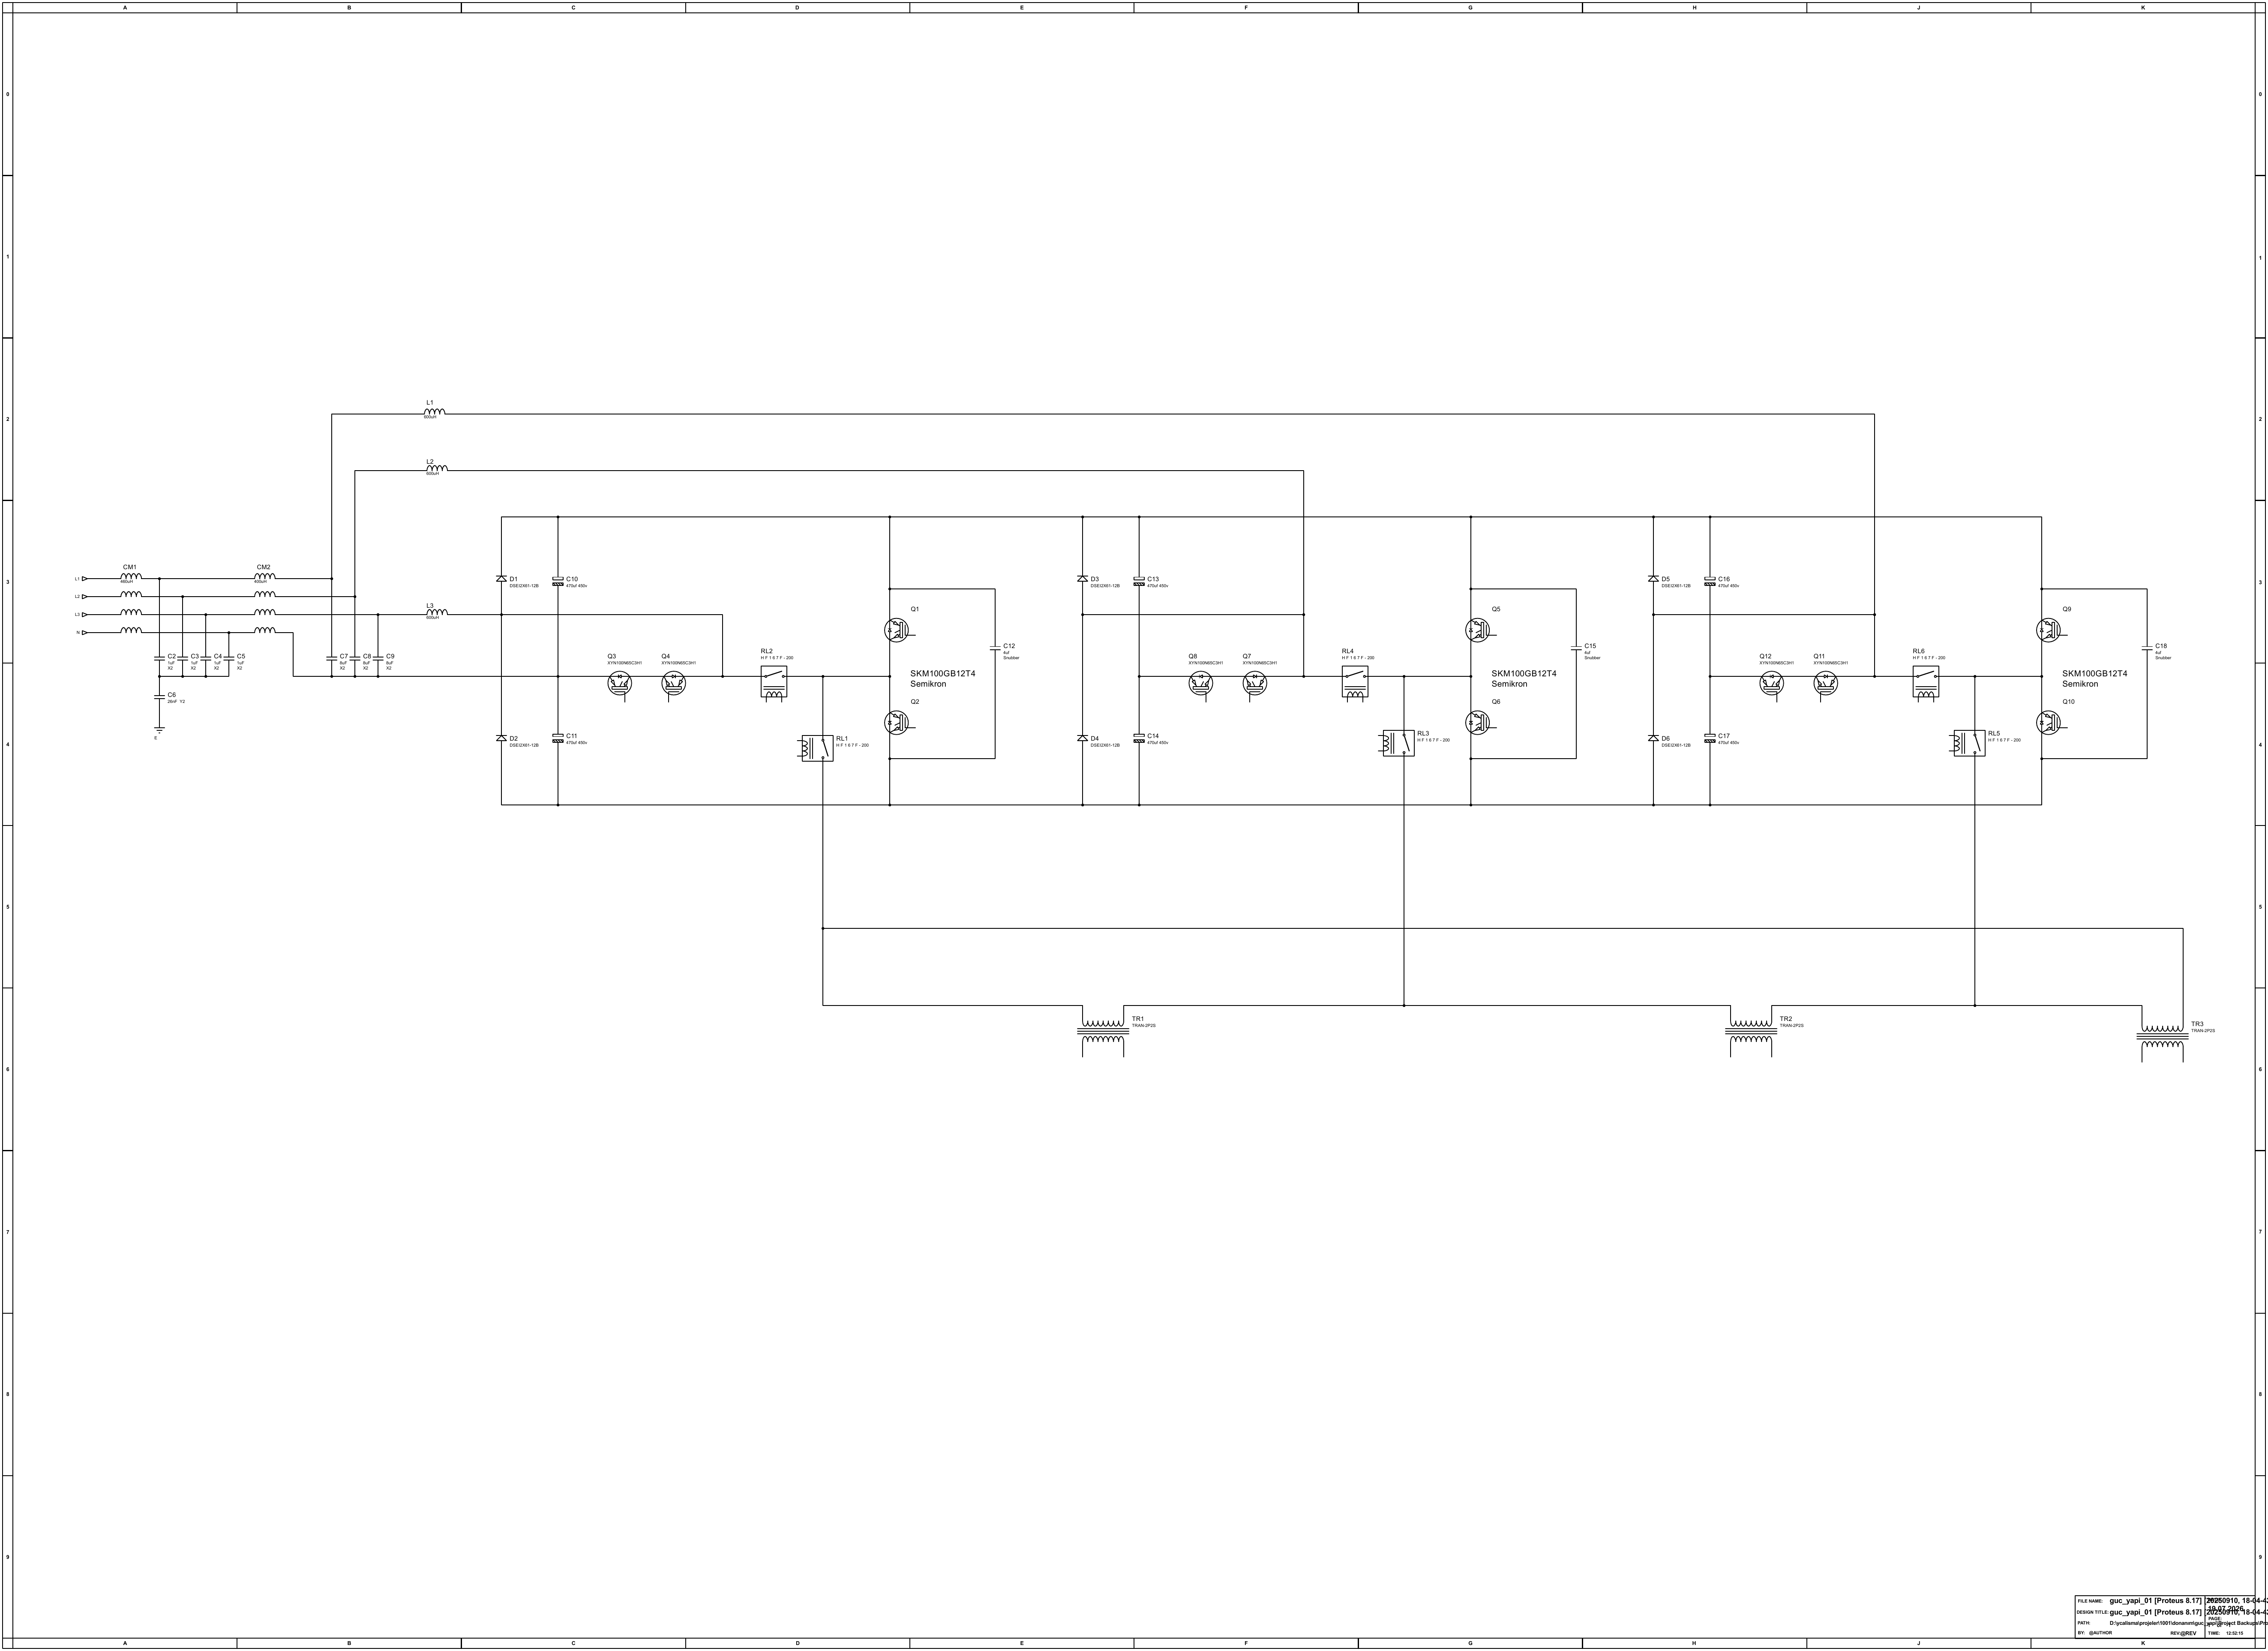
\includegraphics[width=\textwidth]{sistem/tam_topoloji_20260822.png}
  \caption{\juriistegietiketi\ Sonradan sağlanan üç fazlı tam güç topolojisi: ortak giriş/EMI ağı, üç tekrarlı T-tipi faz hücresi, akım algılama--röle yolları ve gerilim algılama transformatörleri. Şema yöntem bölümünde sistem sınırı ve faz-başına indirgeme kaynağı olarak kullanılmıştır.}
  \label{fig:gelen-tam-topoloji}
\end{figure}

Faz indisi $x\in\{a,b,c\}$, DA bara orta noktası $N$, faz kutup gerilimi $v_{xN}$ ve gerilim durumunu seçen boyutsuz anahtarlama değişkeni $s_x\in\{-1,0,1\}$ ile gösterilsin. Üç gerilim durumu
\begin{equation}
  v_{xN}=s_x\frac{V_{\mathrm{dc}}}{2}
  \label{eq:t-tipi-anahtarlama-fonksiyonu}
\end{equation}
biçiminde ortak bir gösterime indirgenebilir. Eşitlik~\eqref{eq:t-tipi-anahtarlama-fonksiyonu}, $s_x=1$, $0$ ve $-1$ için sırasıyla pozitif, sıfır ve negatif kutup gerilimini verir. Doğrusal modülasyon bölgesinde normalize faz komutu $m_x=2v_x^{\ast}/V_{\mathrm{dc}}$ olmak üzere pozitif, negatif ve sıfır durumlarının boyutsuz ideal görev oranları $d_P$, $d_N$ ve $d_O$
\begin{equation}
  d_P=\max(m_x,0),\qquad
  d_N=\max(-m_x,0),\qquad
  d_O=1-|m_x|,\qquad |m_x|\leq 1
  \label{eq:t-tipi-gorev-oranlari}
\end{equation}
olarak yazılabilir \citep{Holmes2003,Wang2020}. Eşitlik~\ref{eq:t-tipi-gorev-oranlari}, modülasyon komutunun genliği azaldığında sıfır durumunun payının neden arttığını doğrudan göstermektedir. Gerçek taşıyıcı tabanlı PWM'de örnekleme, minimum darbe, ölü zaman ve nötr nokta dengeleme müdahaleleri ideal görev oranlarını değiştirebilir; söz konusu etkiler kapı kodu doğrulamasında ayrıca ele alınacaktır.

Eski tezde üç gerilim seviyesi ayrı devre çizimleriyle açıklanmıştır. Şekil~\ref{fig:t-tipi-uc-seviye}, söz konusu çizimleri tek karşılaştırmalı görünüm altında birleştirmektedir. Aynı devre tabanının korunması, hangi anahtarlama durumunun yalnızca bağlantı noktasını değiştirdiğini görmeyi kolaylaştırmaktadır.

\begin{figure}[htbp]
  \centering
  \begin{subfigure}[t]{0.32\textwidth}
    \centering
    \resizebox{\linewidth}{!}{\ttypevector{green!55!black}{gray!65}{gray!65}{gray!65}{%
      \draw[activepath] (4,5) -- (q1.north);
      \draw[activepath] (q1.south) -- (out) -- (5.0,2);}}
    \caption{$P$: $+V_{\mathrm{dc}}/2$}
  \end{subfigure}\hfill
  \begin{subfigure}[t]{0.32\textwidth}
    \centering
    \resizebox{\linewidth}{!}{\ttypevector{gray!65}{gray!65}{green!55!black}{green!55!black}{%
      \draw[activepath] (0,2) -- (q3.west);
      \draw[activepath] (q3.east) -- (q4.west);
      \draw[activepath] (q4.east) -- (out) -- (5.0,2);}}
    \caption{$O$: $0$}
  \end{subfigure}\hfill
  \begin{subfigure}[t]{0.32\textwidth}
    \centering
    \resizebox{\linewidth}{!}{\ttypevector{gray!65}{green!55!black}{gray!65}{gray!65}{%
      \draw[activepath] (4,-1) -- (q2.south);
      \draw[activepath] (q2.north) -- (out) -- (5.0,2);}}
    \caption{$N$: $-V_{\mathrm{dc}}/2$}
  \end{subfigure}
  \caption{\eskitezetiketi\ \juriistegietiketi\ Önceki tezin Şekil~3.2--3.4 çizimlerinden yeniden düzenlenen T-tipi faz kolunun üç gerilim durumu. Yeşil anahtarlar ve mavi bağlantılar ilgili durumun etkin elemanlarını göstermektedir.}
  \label{fig:t-tipi-uc-seviye}
\end{figure}

Tablo~\ref{tab:t-tipi-durumlar}, eski tezdeki devre çizimlerinden çıkarılan kapı durumlarını literatürdeki üç seviyeli gösterimle birlikte özetlemektedir \citep{Holmes2003,Wang2020}. ``1'' iletim komutunu, ``0'' kesim komutunu ifade etmektedir. Tablo yalnızca ideal kararlı durumları göstermekte; ölü zaman sırasında diyot iletimi ve akım yönüne bağlı geçici komütasyon yolları kapsam dışı bırakılmaktadır.

\begin{table}[htbp]
  \centering
  \caption{\eskitezetiketi\ \diskaynaketiketi\ \juriistegietiketi\ T-tipi faz kolunun ideal anahtarlama durumları ve kapı komutları.}
  \label{tab:t-tipi-durumlar}
  \small
  \begin{tabularx}{\textwidth}{c c c c c c X}
    \toprule
    Durum & $Q_1$ & $Q_2$ & $Q_3$ & $Q_4$ & $v_{xN}$ & İşlevsel açıklama \\
    \midrule
    $P$ & 1 & 0 & 1 & 0 & $+V_{\mathrm{dc}}/2$ & Pozitif yarım periyotta enerji üst DA bara kolundan faz çıkışına aktarılır. \\
    $O$ & 0 & 0 & 1 & 1 & $0$ & Faz çıkışı nötr kola bağlanır; filtre akımının yönüne göre serbest dolaşım yolu oluşur. \\
    $N$ & 0 & 1 & 0 & 1 & $-V_{\mathrm{dc}}/2$ & Negatif yarım periyotta enerji alt DA bara kolu üzerinden aktarılır. \\
    \bottomrule
  \end{tabularx}
\end{table}

$P$ durumunda $Q_3$ ve $N$ durumunda $Q_4$ için verilen iletim komutu, eski tezde kullanılan yarım periyot etkinleştirme kuralını yansıtmaktadır; ilgili nötr anahtar aktif enerji yolunda akım taşımamaktadır. Yalnızca gerilim seviyesini üreten asgari durum gösterilecekse $P$ için $Q_1$, $O$ için $Q_3$--$Q_4$ ve $N$ için $Q_2$ iletimde kabul edilebilir. Nihai kapı tablosu, gerçek PWM kodundaki komut dizisiyle karşılaştırılarak bu iki gösterimden hangisinin kullanıldığı açıkça belirtilecektir.

\begin{center}
\juriistegietiketi\ \small Anahtar adları, gerilim seviyesi ve akım yolu tek tabloda eşleştirilmiştir; nihai vektör devrelerde aynı renk lejandı korunacaktır.
\end{center}

Pozitif yarım periyotta modülasyon, $P$ ve $O$ durumları arasında; negatif yarım periyotta ise $N$ ve $O$ durumları arasında yapılır. Endüktif çıkış filtresi nedeniyle faz akımı anahtarlama anında sürekliliğini korur. Gerilim komutu değişse bile akımın mevcut yönü, aktif anahtarın kanalı veya antiparalel diyot üzerinden uygun serbest dolaşım yolunu belirler. Dolayısıyla yalnızca kapı komutlarına bakmak gerçek iletimde bulunan yarı iletkeni tanımlamak için yeterli değildir.

Şekil~\ref{fig:t-tipi-akim-yollari}(a), eski tezin devre çizimlerindeki $C_A$--$C_B$ bölünmüş DA barayı, antiparalel diyotlu $Q_1$--$Q_4$ IGBT'lerini ve faz başına $L_1$--$C_f$--$L_2$ filtresini tek topolojide birleştirmektedir. Eski çizimde $C$ olarak adlandırılan filtre kapasitörü, bölümdeki durum modeliyle tutarlılık için $C_f$ olarak gösterilmiştir. Şekil~\ref{fig:t-tipi-akim-yollari}(b)--(e), aynı güç katının dört temel iletim yolunu karşılaştırmaktadır; akım yolu okunabilirliğini korumak için filtre elemanları alt çizimlerde tekrarlanmamıştır. Pozitif alternansın aktif durumunda $Q_1$ üzerinden, sıfır durumunda nötr kol üzerinden akış gerçekleşir. Negatif alternansta aynı işleyiş alt kol için simetrik biçimde oluşur. Nötr seviyesinde geçirilen sürenin modülasyon indeksi azaldıkça artması, düşük güçte nötr anahtarların iletim payını ve ters akım riskini büyütmektedir.

\begin{figure}[htbp]
  \centering
  \begin{subfigure}[t]{0.96\textwidth}
    \centering
    \resizebox{0.98\linewidth}{!}{\ttypefulltopology}
    \caption{Faz başına tam güç topolojisi ve LCL filtre}
  \end{subfigure}

  \vspace{4mm}
  \begin{subfigure}[t]{0.48\textwidth}
    \centering
    \ttypevector{green!55!black}{gray!65}{gray!65}{gray!65}{%
      \draw[current] (0.7,5) -- (q1.north);
      \draw[current] (q1.south) -- (out) -- (5.0,2);}
    \caption{Pozitif alternans, aktif $P$ durumu}
  \end{subfigure}\hfill
  \begin{subfigure}[t]{0.48\textwidth}
    \centering
    \ttypevector{gray!65}{gray!65}{green!55!black}{green!55!black}{%
      \draw[current] (0.5,2) -- (q3.west);
      \draw[current] (q3.east) -- (q4.west);
      \draw[current] (q4.east) -- (5.0,2);}
    \caption{Pozitif alternans, sıfır $O$ durumu}
  \end{subfigure}

  \vspace{4mm}
  \begin{subfigure}[t]{0.48\textwidth}
    \centering
    \ttypevector{gray!65}{green!55!black}{gray!65}{gray!65}{%
      \draw[current] (5.0,2) -- (out) -- (q2.north);
      \draw[current] (q2.south) -- (0.7,-1);}
    \caption{Negatif alternans, aktif $N$ durumu}
  \end{subfigure}\hfill
  \begin{subfigure}[t]{0.48\textwidth}
    \centering
    \ttypevector{gray!65}{gray!65}{green!55!black}{green!55!black}{%
      \draw[current] (5.0,2) -- (q4.east);
      \draw[current] (q4.west) -- (q3.east);
      \draw[current] (q3.west) -- (0.5,2);}
    \caption{Negatif alternans, sıfır $O$ durumu}
  \end{subfigure}
  \caption{\eskitezetiketi\ \juriistegietiketi\ Önceki tezin T-tipi devre ve Şekil~3.5--3.8 akım yolu çizimlerinin ortak devre dili ve renk lejandıyla vektörel yeniden düzenlenmesi. Tam topoloji $C_A$, $C_B$, antiparalel diyotlu IGBT'ler, $L_1$, $C_f$ ve $L_2$ elemanlarını; kırmızı oklar ise tanımlanan pozitif akım yönüne göre iletim yollarını göstermektedir.}
  \label{fig:t-tipi-akim-yollari}
\end{figure}

\begin{samepage}
  Şekil~\ref{fig:t-tipi-akim-yollari}(a), faz kolunun işlevsel güç topolojisidir; kart üretim veya bağlantı şeması niteliği taşımamaktadır. Kapı sürücüleri, sensörler, koruma devreleri, konektörler, yarı iletken parça kodları ve kesin pasif eleman değerlerini içeren ayrıntılı uygulama şeması, gerçek donanım kaydıyla doğrulandıktan sonra Ek~A'da verilecektir.

  \begin{center}
  \juriistegietiketi\ \small Jürinin çalışma modlarının tek devre tabanı üzerinde anlaşılır gösterilmesi talebi uygulanmıştır: etkin anahtarlar yeşil, pasif anahtarlar gri, gerilim durumu mavi ve akım yönü kırmızı kullanılmıştır.
  \end{center}
\end{samepage}

\tezcalismanotu{D3-1 --- Eski topoloji şekillerinin uygulama devresiyle doğrulanması}{Eski Şekil~3.2--3.8 ortak vektör devrelerde birleştirilmiş, akım yolları aynı çizim tabanında gösterilmiştir. Sonradan gelen tam topolojiyle faz bobinlerinin ve güç yarı iletkenlerinin yerleşimi doğrulanmış; filtre seti $L_1=\SI{600}{\micro\henry}$, $C_f=\SI{8}{\micro\farad}$ ve $L_2=\SI{200}{\micro\henry}$ olarak kaynak ayrıştırmasıyla kilitlenmiştir. Buna karşılık $C_A$--$C_B$ bara bağlantısının bütün ayrıntıları, sürücü/koruma elemanları ve gerçek PWM--ölü zaman uygulaması eksiksiz BOM ve kontrol koduyla doğrulanmayı sürdürmektedir.}

\section{Düşük Güç Eşdeğeri ve Ters Akım Mekanizması}

Faz gerilimi referansının genliği azaldığında aktif $P$ veya $N$ durumunun görev oranı küçülür, sıfır durumunun süresi uzar. Pozitif ve negatif yarım periyotlar ayrı ayrı ele alındığında faz kolu, anahtarlanan gerilim kaynağı ile filtre endüktansı bakımından senkron alçaltıcı dönüştürücüye eşdeğer bir davranış gösterir \citep{Mohan2003,Erickson2001}. Eski tezde önerilen eşdeğerler Şekil~\ref{fig:senkron-buck-esdeger} altında bir araya getirilmiştir.

\begin{figure}[htbp]
  \centering
  \begin{subfigure}[t]{0.46\textwidth}
    \centering
    \resizebox{\linewidth}{!}{\syncbuckvector{$+V_{\mathrm{dc}}/2$}{$N$}{$Q_1$}{$Q_3$}}
    \caption{Pozitif yarım periyot eşdeğeri}
  \end{subfigure}\hfill
  \begin{subfigure}[t]{0.46\textwidth}
    \centering
    \resizebox{\linewidth}{!}{\syncbuckvector{$N$}{$-V_{\mathrm{dc}}/2$}{$Q_4$}{$Q_2$}}
    \caption{Negatif yarım periyot eşdeğeri}
  \end{subfigure}
  \caption{\eskitezetiketi\ \juriistegietiketi\ Önceki tezin Şekil~3.9--3.10 çizimlerinden vektörel olarak yeniden düzenlenen T-tipi faz kolunun yarım periyotlara göre senkron-buck eşdeğerleri. Yeşil anahtar ve mavi yol aktif enerji aktarımını göstermektedir.}
  \label{fig:senkron-buck-esdeger}
\end{figure}

Anahtarlama periyodu $T_{\mathrm{s}}$, boyutsuz görev oranı $d\in[0,1]$, faz koluna uygulanan etkin DA gerilimi $V_{\mathrm{h}}$, anık şebeke gerilimi $v_{\mathrm{g}}$, eşdeğer filtre endüktansı $L$ ve anahtarın iletim/kesim aralıklarındaki endüktör gerilimleri $v_{L,\mathrm{on}}$ ile $v_{L,\mathrm{off}}$ olarak tanımlansın. Pozitif yarım periyotta ideal gerilimler
\begin{equation}
  \begin{aligned}
    v_{L,\mathrm{on}} &= V_{\mathrm{h}}-v_{\mathrm{g}}, \\
    v_{L,\mathrm{off}} &= -v_{\mathrm{g}}
  \end{aligned}
  \label{eq:buck-enduktor-gerilimleri}
\end{equation}
biçimindedir. Eşitlik~\eqref{eq:buck-enduktor-gerilimleri} altında anahtarlama periyodu boyunca gerilimlerin yaklaşık sabit kaldığı ve yerel kararlı durumda volt--saniye dengesinin sağlandığı kabul edilirse tepe--tepe akım dalgalanması $\Delta i_L$
\begin{equation}
  \Delta i_L \simeq \frac{(V_{\mathrm{h}}-v_{\mathrm{g}})dT_{\mathrm{s}}}{L}
  =\frac{v_{\mathrm{g}}(1-d)T_{\mathrm{s}}}{L}
  \label{eq:buck-akim-dalgalanmasi}
\end{equation}
ile bulunur \citep{Erickson2001,Chen2010}. Eşitlik~\eqref{eq:buck-akim-dalgalanmasi} içindeki iki ifade yalnızca aynı yerel volt--saniye dengesi altında eşdeğerdir. Ortalama akım $\bar{i}_L$ değerinin dalgalanmanın yarısından küçük olduğu bölgede akım sıfırı geçebilir:
\begin{equation}
  \bar{i}_L < \frac{\Delta i_L}{2}.
  \label{eq:ters-akim-esigi}
\end{equation}
Senkron anahtar sıfır geçişinden sonra iletimde tutulursa $i_L<0$ aralığı oluşur ve filtredeki enerji DA tarafa geri taşınır. Yararlı çıkış gücüne katkı sağlamayan söz konusu dolaşım, RMS akımı ile iletim kayıplarını artırabilir. Diyot benzetimi yaklaşımı, akım sıfıra yaklaştığında senkron yolu keserek negatif akımı engeller; sıfır akım algılamadaki gecikme ve anahtarlama geçişleri ise gerçek kayıp sınırını belirler \citep{Chen2010,Erickson2001}.

Birincil kaynaktaki diyot benzetimi--sürekli iletim karşılaştırması Şekil~\ref{fig:de-ccm-akim} üzerinde Bölüm~2'de verilmiştir. Önceki tezin Şekil~3.11 ve Şekil~3.12'sindeki açıklayıcı şemalar da aynı kuramsal anlatım altında Şekil~\ref{fig:onceki-tez-ccm-ters-akim} ve Şekil~\ref{fig:onceki-tez-dcm-akim} olarak Bölüm~2'ye taşınmıştır. Mevcut bölüm, söz konusu genel senkron-buck davranışını Eşitlik~\ref{eq:ters-akim-esigi} ile T-tipi faz koluna uyarlamaktadır.

T-tipi faz kolunda nötr anahtarların susturulması benzer bir amaç taşımaktadır: düşük güçte, referans akım yönüne ters enerji dolaşımı oluşturan komütasyonların azaltılması hedeflenir. Yaklaşım, klasik PWM'nin bütün çalışma aralığında değiştirilmesi yerine belirlenen düşük güç veya küçük modülasyon bölgesinde etkinleştirilmelidir. Eşik seçimi yalnızca akım genliğine bağlanamaz; akım dalgalanması, ölçüm gürültüsü, ölü zaman, şebeke gerilimi ve hesaplama gecikmesi de karar mantığına dâhil edilmelidir.

\section{LCL Filtre ve Şebeke Modeli}

Şebeke bağlantılı eviricide LCL filtre, anahtarlama frekansı çevresindeki gerilim bileşenlerini daha küçük toplam endüktansla bastırabilmektedir. Rezonans tepesi ve şebeke empedansına duyarlılık, filtreyi yalnızca pasif bir zayıflatıcı olmaktan çıkarıp kapalı çevrim tasarımının parçası hâline getirir \citep{Zhang2014PR,Lu2016}. Faz başına ortalama modelde evirici tarafı endüktansı $L_1$, filtre kapasitörü $C_f$, şebeke tarafı endüktansı $L_2$, seri kayıplar $R_1$ ve $R_2$ ile gösterilmiştir. Şebeke eşdeğer endüktansı gerektiğinde $L_2$ içine eklenmektedir.

Şekil~\ref{fig:faz-basina-lcl-modeli}, durum denklemlerinde kullanılan işaretleri fiziksel ölçüm noktalarıyla eşleştirmektedir. $i_1$ evirici tarafı endüktör akımını, $i_2$ ortak bağlantı noktasına aktarılan şebeke akımını ve $v_c$ filtre kapasitörü gerilimini göstermektedir. Gerçek donanımda ölçülen akımın $i_1$ veya $i_2$ olması, denetleyici bitki modelini ve aktif sönümleme yolunu değiştireceğinden sensör konumu kod ve devre şemasıyla kesinleştirilecektir.

\begin{figure}[htbp]
  \centering
  \resizebox{0.96\textwidth}{!}{%
  \begin{tikzpicture}[
    block/.style={draw,rounded corners=1pt,minimum width=13mm,minimum height=8mm,fill=blue!4},
    resistor/.style={draw,minimum width=8mm,minimum height=5mm,fill=white},
    coilpath/.style={decorate,decoration={coil,aspect=0.48,segment length=2.9mm,amplitude=1.9mm}},
    sensor/.style={circle,draw,fill=orange!10,minimum size=7mm,font=\scriptsize},
    flow/.style={-{Latex[length=2mm]},line width=1.0pt},
    current/.style={-{Latex[length=2mm]},red!80!black,line width=1.0pt},
    wire/.style={line width=0.9pt},
    signal/.style={-{Latex[length=1.8mm]},dashed,gray!80}
  ]
    \node[block,align=center] (inv) at (0,0) {T-tipi\\faz kolu};
    \node[resistor] (r1) at (1.65,0) {$R_1$};
    \coordinate (l1a) at (2.35,0);
    \coordinate (l1b) at (3.45,0);
    \coordinate (vc) at (4.10,0);
    \node[resistor] (r2) at (5.30,0) {$R_2$};
    \coordinate (l2a) at (5.95,0);
    \coordinate (l2b) at (7.05,0);
    \node[block,align=center] (grid) at (8.55,0) {Şebeke\\$v_g$};
    \draw[wire] (inv.east) -- node[above,font=\scriptsize] {$v_{\mathrm{inv}}$} (r1.west);
    \draw[wire] (r1.east) -- (l1a);
    \draw[coilpath,line width=0.9pt] (l1a) -- (l1b);
    \draw[wire] (l1b) -- (vc) -- (r2.west);
    \draw[wire] (r2.east) -- (l2a);
    \draw[coilpath,line width=0.9pt] (l2a) -- (l2b);
    \draw[wire] (l2b) -- (grid.west);
    \node[above=2mm,font=\scriptsize] at ($(l1a)!0.5!(l1b)$) {$L_1$};
    \node[above=2mm,font=\scriptsize] at ($(l2a)!0.5!(l2b)$) {$L_2$};
    \draw[current] (2.30,0.55) -- node[above,font=\scriptsize] {$i_1$} (3.45,0.55);
    \draw[current] (5.90,0.55) -- node[above,font=\scriptsize] {$i_2$} (7.05,0.55);
    \fill (vc) circle (1.6pt);
    \draw[line width=0.8pt] (vc) -- (4.10,-0.8);
    \draw[line width=0.8pt] (3.73,-0.8) -- (4.47,-0.8);
    \draw[line width=0.8pt] (3.73,-1.08) -- (4.47,-1.08);
    \draw[line width=0.8pt] (4.10,-1.08) -- (4.10,-1.50);
    \draw[line width=0.8pt] (3.73,-1.50) -- (4.47,-1.50);
    \draw[line width=0.8pt] (3.83,-1.65) -- (4.37,-1.65);
    \draw[line width=0.8pt] (3.95,-1.80) -- (4.25,-1.80);
    \node[right,font=\scriptsize] at (4.40,-0.94) {$C_f$};
    \node[above,font=\scriptsize] at (vc) {$v_c$};
    \node[sensor] (si1) at (2.90,-2.25) {$i_1$};
    \node[sensor] (svc) at (4.10,-2.25) {$v_c$};
    \node[sensor] (si2) at (6.50,-2.25) {$i_2$};
    \node[block,fill=gray!8,align=center] (adc) at (4.85,-3.55) {Ölçüm ve\\ADC zinciri};
    \draw[signal] ($(l1a)!0.5!(l1b)$) -- (si1.north);
    \draw[signal] (vc) -- (svc.north);
    \draw[signal] ($(l2a)!0.5!(l2b)$) -- (si2.north);
    \draw[signal] (si1) -- (adc);
    \draw[signal] (svc) -- (adc);
    \draw[signal] (si2) -- (adc);
  \end{tikzpicture}%
  }
  \caption{\juriistegietiketi\ Faz başına LCL filtre, durum değişkenleri ve denetimde kullanılacak aday ölçüm noktaları.}
  \label{fig:faz-basina-lcl-modeli}
\end{figure}

Evirici kutup gerilimi $v_{\mathrm{inv}}$, kapasitör gerilimi $v_c$, şebeke gerilimi $v_g$, evirici tarafı akımı $i_1$ ve şebeke akımı $i_2$ için durum denklemleri
\begin{equation}
  \begin{aligned}
    L_1\frac{\mathrm{d}i_1}{\mathrm{d}t} &= v_{\mathrm{inv}}-v_c-R_1i_1, \\
    C_f\frac{\mathrm{d}v_c}{\mathrm{d}t} &= i_1-i_2, \\
    L_2\frac{\mathrm{d}i_2}{\mathrm{d}t} &= v_c-v_g-R_2i_2
  \end{aligned}
  \label{eq:lcl-durum-denklemleri}
\end{equation}
olarak elde edilir. Eşitlik~\eqref{eq:lcl-durum-denklemleri} içindeki $L_1$, $L_2$ ve $C_f$ enerji depolayan filtre elemanlarını; $R_1$ ile $R_2$ seri eşdeğer kayıpları temsil eder. Laplace değişkeni $s$, $i_2(t)$ ve $v_{\mathrm{inv}}(t)$ işaretlerinin Laplace dönüşümleri sırasıyla $I_2(s)$ ve $V_{\mathrm{inv}}(s)$ olarak tanımlansın. Kayıpların ihmal edildiği modelde $v_g=0$ alınarak modülasyon geriliminden şebeke akımına aktarım
\begin{equation}
  G_{vi}(s)=\frac{I_2(s)}{V_{\mathrm{inv}}(s)}
  =\frac{1}{L_1L_2C_fs^3+(L_1+L_2)s}
  \label{eq:lcl-aktarim}
\end{equation}
şeklindedir. Eşitlik~\eqref{eq:lcl-aktarim} kayıpsız ve şebeke gerilimi bozucusu sıfırlanmış ideal bitkiyi tanımlar. Rezonans açısal frekansı $\omega_r$ ve hertz cinsinden rezonans frekansı $f_r$
\begin{equation}
  \omega_r=\sqrt{\frac{L_1+L_2}{L_1L_2C_f}},
  \qquad f_r=\frac{\omega_r}{2\pi}
  \label{eq:lcl-rezonans}
\end{equation}
ile hesaplanır. Eşitlik~\eqref{eq:lcl-rezonans}, seri kayıpları ve ek sönümleme kolunu içermeyen ideal LCL sonucudur. Gerçek modelde seri dirençler, kapasitör sönümleme kolu, sayısal gecikme ve şebeke empedansı aktarım fonksiyonuna eklenmelidir. Kararlılık incelemesinde kullanılan $L(s)$, $S(s)$ ve $T(s)$ fonksiyonları bu fiziksel model üzerinden üretilecek; yalnızca ideal LCL ifadesinden çizilen Bode grafiği nihai kanıt sayılmayacaktır.

\begin{center}
\juriistegietiketi\ \small Sin\textsuperscript{3} yöntemi için kapalı çevrim ve Bode analizi Bölüm 5'te; ideal model, gerçek gecikmeler, $L$--$S$--$T$ eğrileri, kazanç/faz marjları ve birden fazla çalışma noktasıyla verilecektir.
\end{center}

\section{Denetim, Modülasyon ve Sin\texorpdfstring{\textsuperscript{3}}{3} Kompanzasyonu}

Akım döngüsü, referans akım $i^{\ast}$ ile ölçülen şebeke veya evirici tarafı akımı arasındaki hatadan modülasyon komutu üretir. PR denetleyicisinin aktarımı $C_i(s)$, oransal kazanç $K_p$, rezonans kazanç $K_r$, şebeke temel açısal frekansı $\omega_0$ ve pratik rezonans bandını belirleyen pozitif bant katsayısı $\omega_c$ ile gösterilsin. Sinüzoidal referansın kalıcı durum hatasını azaltmak için kullanılabilecek genel yapı
\begin{equation}
  C_i(s)=K_p+\frac{2K_r\omega_c s}{s^2+2\omega_c s+\omega_0^2}
  \label{eq:pr-denetleyici}
\end{equation}
biçiminde gösterilebilir \citep{Teodorescu2006PR,Zhang2014PR}. Eşitlik~\eqref{eq:pr-denetleyici} içindeki $\omega_c$, ideal sonsuz kazançlı rezonatör yerine sonlu bantlı uygulama modelini verir. Tezde kullanılan gerçek denetleyici yapısı, yazılım kodu ve parametre kayıtlarıyla doğrulandıktan sonra denklem ve parametre tablosunda kesinleştirilecektir.

Referans ve ölçülen akımların Laplace dönüşümleri $I^{\ast}(s)$ ile $I(s)$; normalize toplam modülasyon komutu, klasik ileri besleme ve Sin\textsuperscript{3} yolu sırasıyla $U_{\mathrm{mod}}^{\ast}(s)$, $U_{\mathrm{ff}}(s)$ ve $U_{\sin^3}(s)$ olarak tanımlansın. Modülasyon komutu kavramsal olarak
\begin{equation}
  U_{\mathrm{mod}}^{\ast}(s)=C_i(s)\left[I^{\ast}(s)-I(s)\right]+U_{\mathrm{ff}}(s)+U_{\sin^3}(s)
  \label{eq:modulasyon-toplami}
\end{equation}
şeklinde ayrılmıştır. Eşitlik~\eqref{eq:modulasyon-toplami} zaman alanı işaretleriyle aktarım fonksiyonunu aynı ifadede karıştırmamak için tamamen Laplace alanında yazılmıştır. $U_{\mathrm{ff}}$ şebeke gerilimi veya bozucu bastırma amacıyla kullanılan klasik ileri besleme terimini, $U_{\sin^3}$ ise önerilen ikincil şekillendirmeyi temsil eder. PLL faz açısı $\theta$ için trigonometrik özdeşlik
\begin{equation}
  \sin^3(\theta)=\frac{3\sin(\theta)-\sin(3\theta)}{4}
  \label{eq:sin3-ozdeslik}
\end{equation}
kompanzasyonun temel ve üçüncü harmonik bileşenlerini açıkça göstermektedir. Eşitlik~\eqref{eq:sin3-ozdeslik} içindeki $\theta$ boyutsuz elektriksel açıdır. Katsayı ve işaret, gözlenen üçüncü harmonik bozulumunu azaltacak biçimde belirlenmeli; terim doygunluk ve modülasyon sınırlarından önce uygun sınırlayıcılarla uygulanmalıdır.

Önceki tezin Şekil~3.14--3.16 anlatımında akım hatası, denetleyici çıkışı ve anahtar konumları temsili dalga biçimleriyle ilişkilendirilmiştir. Ham model bulunmadığı için söz konusu raster grafikler yöntem kanıtı olarak doğrudan aktarılmamış; içerdiği işlevsel ilişki Şekil~\ref{fig:denetim-modulasyon-blok} üzerinde ölçümden kapı işaretine uzanan izlenebilir bir blok yapısına dönüştürülmüştür. Yapı, Sin\textsuperscript{3} yolunun akım denetleyicisiyle seri değil modülasyon toplamında paralel bir ileri besleme bileşeni olduğunu ve nötr anahtar susturma kararının PWM üretiminden sonra kapı mantığında uygulandığını açıkça ayırmaktadır.

\begin{figure}[H]
  \centering
  \resizebox{0.99\textwidth}{!}{%
  \begin{tikzpicture}[
    node distance=5mm and 5mm,
    block/.style={draw,rounded corners=1.3pt,align=center,minimum height=9mm,minimum width=14mm,fill=blue!5},
    special/.style={draw,rounded corners=1.3pt,align=center,minimum height=9mm,minimum width=18mm,fill=orange!12},
    sum/.style={circle,draw,minimum size=7mm,inner sep=0pt},
    flow/.style={-{Latex[length=1.8mm]},line width=0.9pt},
    feedback/.style={-{Latex[length=1.8mm]},line width=0.9pt,dashed}
  ]
    \node[block] (iref) {$i^{\ast}$\\üretimi};
    \node[sum,right=of iref] (sumi) {$\Sigma$};
    \node[block,right=of sumi] (ci) {$C_i(s)$\\akım denetimi};
    \node[sum,right=of ci] (sumv) {$\Sigma$};
    \node[block,right=of sumv,minimum width=24mm] (pwm) {Sınırlandırma, ölçekleme\\ve PWM üretimi};
    \node[special,right=of pwm,minimum width=25mm] (gate) {$Q_1$--$Q_4$ kapı mantığı\\ve nötr susturma};
    \node[block,right=of gate,minimum width=20mm] (plant) {T-tipi güç katı\\ve LCL filtre};
    \draw[flow] (iref) -- (sumi);
    \draw[flow] (sumi) -- node[above,font=\scriptsize] {$e_i$} (ci);
    \draw[flow] (ci) -- (sumv);
    \draw[flow] (sumv) -- node[above,font=\scriptsize] {$v_{\mathrm{mod}}^{\ast}$} (pwm);
    \draw[flow] (pwm) -- (gate);
    \draw[flow] (gate) -- node[above,font=\scriptsize] {$q_1$--$q_4$} (plant);

    \node[special,below=13mm of ci,xshift=-7mm,text width=23mm] (vff) {Şebeke gerilimi\\ileri besleme $v_{\mathrm{ff}}$};
    \node[special,below=13mm of sumv,xshift=11mm,minimum width=20mm] (sin3) {Sin\textsuperscript{3}\\$K_{\sin^3}\sin^3\theta$};
    \node[block,below=11mm of iref] (pll) {Faz bilgisi\\$\theta$};
    \node[block,below=11mm of plant] (meas) {Ölçüm, ADC\\ve ölçekleme};
    \draw[flow] (pll) -- (iref);
    \coordinate (phasebus) at ($(pll.south)+(0,-0.65)$);
    \draw[flow] (pll.south) -- (phasebus) -| (sin3.south);
    \draw[flow] (vff) -| (sumv.south);
    \draw[flow] (sin3) -- (sumv.south);
    \draw[feedback] (plant.south) -- (meas.north);
    \coordinate (feedbackbus) at ($(vff.south)+(0,-1.0)$);
    \draw[feedback] (meas.south) |- (feedbackbus) -| node[pos=0.72,below,font=\scriptsize] {$i_{\mathrm{ölç}}$} (sumi.south);
    \node[font=\scriptsize] at ($(sumi)+(-0.24,0.34)$) {$+$};
    \node[font=\scriptsize] at ($(sumi)+(-0.24,-0.34)$) {$-$};
    \node[font=\scriptsize] at ($(sumv)+(-0.24,0.34)$) {$+$};
    \pgfresetboundingbox
    \coordinate (bboxse) at (meas.east |- feedbackbus);
    \path[use as bounding box] ($(iref.north west)+(-0.3,0.35)$) rectangle ($(bboxse)+(0.3,-0.3)$);
  \end{tikzpicture}%
  }
  \caption{\eskitezetiketi\ \juriistegietiketi\ Önceki tezin denetleyici davranışı açıklamalarından yeniden düzenlenen işlevsel akım denetimi, ileri besleme, Sin\textsuperscript{3}, PWM ve nötr anahtar susturma blokları.}
  \label{fig:denetim-modulasyon-blok}
\end{figure}

\begin{center}
\juriistegietiketi\ \small Bölümsel kontrol blok diyagramı yöntem düzeyinde tamamlanmıştır. Denetleyici türü, işaretler, sınırlayıcı sırası, PWM güncelleme anı ve nötr susturma koşulu gerçek kodla karşılaştırıldığında nihai uygulama ayrıntıları kilitlenecektir.
\end{center}

İdeal doğrusal modelde dışsal ileri besleme terimi karakteristik paydayı değiştirmeyebilir. Sayısal uygulamada örnekleme, sıfırıncı derece tutucu, PWM, hesaplama ve ölçüm filtreleri toplam bir gecikme $G_d(s)$ oluşturur. Şekil~\ref{fig:denetim-modulasyon-blok} içindeki küçük harfli $v_{\mathrm{ff}}(t)$, $v_{\sin^3}(t)$ ve $v_{\mathrm{mod}}^{\ast}(t)$ zaman alanındaki fiziksel/normalize komutları; Eşitlik~\eqref{eq:modulasyon-toplami} içindeki büyük harfler aynı işaretlerin Laplace dönüşümlerini gösterir. Şebeke gerilimi ileri beslemesinin LCL rezonansında pozitif veya negatif sönümleme üretmesi mümkün olduğundan iki ileri besleme yolu kapalı çevrim analizinde ayrı girişler olarak tutulacaktır \citep{Lu2016,Wang2024}. Dolayısıyla Sin\textsuperscript{3} teriminin başarısı yalnızca düşük güç THD değeriyle değil, akım izleme hatası, kararlılık marjı, kontrol eforu, doyum süresi ve anma gücündeki etkisizliği veya güvenli katkısı ile birlikte değerlendirilecektir.

\tezcalismanotu{D3-2 --- Eski Şekil 3.13--3.16 ve denetim bloğunun yeniden üretimi}{Senaryo~1 `.slx` modeli alınmış, ancak R2025b'de kaldırılan bloklar nedeniyle kaynak koşu tamamlanamamış; Senaryo~2--4 kontrol kodu gelmemiştir. Aynı dört işaretin ortak zaman tabanında üretilmesi için kaynak modelin doğrulanmış dönüşümü ile denetleyici türü, işaret yönleri, sınırlayıcı sırası, PWM güncelleme anı, kapı eşlemesi ve nötr susturma koşulu gereklidir. Bölüm~5'teki yeni koşular yöntem fizibilitesi sağlar, özgün kodun bire bir yeniden üretimi değildir.}

\section{Elektriksel ve Denetim Parametreleri}

Eski tezdeki elektriksel değerler topoloji, gerçek zamanlı uygulama ve ölçüm alt başlıklarına dağılmıştır. Tablo~\ref{tab:sistem-parametreleri}, jüri talebi doğrultusunda doğrulanabilen bilgileri tek yerde toplamakta ve eksik kayıtları görünür kılmaktadır. ``DOĞRULANACAK'' ifadesi bilinmeyen değeri tahminle doldurmak yerine, kod, şema, bobin etiketi, ölçüm dosyası veya danışman onayı gerektiren alanı göstermektedir.

\begin{longtable}{>{\raggedright\arraybackslash}p{0.26\textwidth} >{\raggedright\arraybackslash}p{0.24\textwidth} >{\raggedright\arraybackslash}p{0.39\textwidth}}
\caption{\eskitezetiketi\ \juriistegietiketi\ Elektriksel, denetim ve ölçüm parametrelerinin birleşik çalışma tablosu.}\label{tab:sistem-parametreleri}\\
\toprule
Parametre & Değer & Durum / doğrulama kaynağı \\
\midrule
\endfirsthead
\toprule
Parametre & Değer & Durum / doğrulama kaynağı \\
\midrule
\endhead
Faz yapısı & Üç faz, dört telli & Eski tez prototip açıklaması; doğrulandı. \\
Tasarım güç aralığı & \SI{20}{\kilo\watt}--\SI{25}{\kilo\watt} & Eski tezde deney düzeneği için verilen tasarım aralığı. \\
Prototip anma gücü & \SI{20}{\kilo\volt\ampere} & Akım sensörü boyutlandırma hesabında verilen değer; kW/kVA adlandırması nihai sürümde kilitlenecek. \\
Şebeke frekansı & \SI{50}{\hertz} & Türkiye şebeke koşulu; deney kaydı veya yazılım PLL ayarıyla doğrulanacak. \\
Şebeke anma gerilimi & \SI{230}{\volt} faz--nötr, \SI{400}{\volt} faz--faz & Donanım tasarım açıklaması; deneyler varyak nedeniyle daha düşük gerilimde yürütülmüş. \\
Deney faz--nötr gerilimi & Yaklaşık \SI{120}{\volt}--\SI{130}{\volt} & Eski tezde karşılaştırmalı düşük güç deneyleri için raporlanan aralık. \\
DA bara gerilimi & Yaklaşık \SI{400}{\volt} & Eski tez genel deney koşulu; ayrı deneylerde \SI{395}{\volt}--\SI{430}{\volt}. Toplam/yarım bara tanımı DOĞRULANACAK. \\
DA bara ölçüm aralığı & \SI{470}{\volt} & AMC1200 giriş bölücüsü için verilen tasarım değeri. \\
Faz RMS akım tasarımı & Yaklaşık \SI{30}{\ampere} & \SI{20}{\kilo\volt\ampere} ve faz başına güç hesabı. \\
Faz RMS akım üst sınırı & Yaklaşık \SI{36}{\ampere} & Yüzde 20 tasarım toleransıyla verilen hedef. \\
Mevcut aşırı akım eşiği & Yaklaşık \SI{30.4}{\ampere} & Pencere karşılaştırıcı ve \SI{23}{\milli\volt\per\ampere} sensör kazancından hesaplanmış. \\
Akım sensörü & HLSR 20-P SP33 & Ölçüm kartı donanım kaydı; ölçülebilir tepe akımı \SI{56.5}{\ampere}. \\
Gerilim ölçümü & AMC1200, 12 bit ADC & Eski tez ölçüm zinciri; \SI{1.3}{\volt} ofset ve \SI{2.6}{\volt} ADC referansı. \\
Sayısal denetleyici & PIC32MK ailesi, 32 bit & Kontrol kartı açıklaması; tam parça kodu DOĞRULANACAK. \\
Anahtarlama frekansı $f_s$ & {\small DOĞRULANACAK} & Eski tez genel anlatımında \SI{5}{\kilo\hertz}--\SI{20}{\kilo\hertz} aralığı geçiyor; gerçek yazılım değeri bulunmadan tek sayı kullanılmayacak. \\
Örnekleme frekansı $f_{\mathrm{samp}}$ & {\small DOĞRULANACAK} & Kontrol yazılımı veya zamanlayıcı yapılandırmasından çıkarılacak. \\
Ölü zaman $t_d$ & {\small DOĞRULANACAK} & Sürücü/PWM yapılandırması ve osiloskop kaydı gerektiriyor. \\
$L_1$, $C_f$, $L_2$ & \SI{600}{\micro\henry}, \SI{8}{\micro\farad}, \SI{200}{\micro\henry} & 26.08.2026 kaynak ayrıştırmasıyla kilitlendi: \SI{600}{\micro\henry} tam topolojide faz başına bobin; \SI{200}{\micro\henry} e-posta ve Excel gerçek uygulama satırlarında ikinci filtre/yük endüktansı; \SI{400}{\micro\henry} ise alınan Senaryo~1 modelindeki eski \texttt{CL1} ayarıdır. \\
PR/akım denetleyici katsayıları & {\small DOĞRULANACAK} & Denetleyici türü ve katsayıları kaynak kodla eşleştirilecek. \\
Sin\textsuperscript{3} kazancı ve etkinleşme eşiği & {\small DOĞRULANACAK} & Benzetim dosyası, deney kodu ve çalışma noktası kayıtları birlikte incelenecek. \\
\bottomrule
\end{longtable}

\begin{center}
\juriistegietiketi\ \small Jürinin tek parametre tablosu talebi karşılandı. Sarı işaret, ilk değerlerin eski tezden derlendiğini; `DOĞRULANACAK' hücreleri ise ham mühendislik kanıtı bekleyen alanları gösterir.
\end{center}

\subsection{Üç Endüktans Değerinin Ayrıştırılması ve $L_2$ Seçimi}

Kaynaklardaki \SI{200}{\micro\henry}, \SI{400}{\micro\henry} ve \SI{600}{\micro\henry} değerleri aynı devre elemanına ait üç ölçüm değildir. En yeni parametre notu $L_2=\SI{200}{\micro\henry}$ vermekte; Excel'deki gerçek uygulama sonuçlarının Senaryo~1 ve Senaryo~2 satırlarında da \texttt{LL [H]} hücresi $0{,}0002$~H olarak bu değeri bağımsız biçimde tekrarlamaktadır. Alınan Senaryo~1 \texttt{.slx} dosyasında, \SI{600}{\micro\henry} evirici tarafı bobin ile \SI{8}{\micro\farad} şönt kapasitörden sonra şebekeye seri bağlı \texttt{CL1} bloğu \SI{400}{\micro\henry} olarak ayarlanmıştır; bu değer kaynak modelin eski yapılandırmasıdır. Tam topolojideki ``L2, \SI{600}{\micro\henry}'' etiketi ise B fazı bobinidir ve aynı şemada A ve C fazı bobinleri de sırasıyla L1 ve L3 adıyla \SI{600}{\micro\henry} değerindedir. Bu nedenle nihai faz-başına LCL seti $L_1=\SI{600}{\micro\henry}$, $C_f=\SI{8}{\micro\farad}$ ve $L_2=\SI{200}{\micro\henry}$ olarak seçilmiştir.

İdeal, kayıpsız LCL rezonansı Eşitlik~\eqref{eq:lcl-rezonans} ile hesaplanmıştır.
Tablo~\ref{tab:l2-aday-karsilastirma}, üç değeri aynı $L_1$, $C_f$, \SI{50}{\hertz} ve kaynak modeldeki \SI{10}{\kilo\hertz} anahtarlama frekansı altında karşılaştırmaktadır. ``\SI{600}{\micro\henry} adayı'' satırı yalnız duyarlılık hesabıdır; tam topolojideki faz etiketi filtre $L_2$'si olarak kabul edilmemiştir.

\begin{table}[htbp]
  \centering
  \caption{Üç endüktans değerinin kaynak, devre rolü ve ideal LCL duyarlılığı bakımından karşılaştırılması.}
  \label{tab:l2-aday-karsilastirma}
  \footnotesize
  \renewcommand{\arraystretch}{1.10}
  \begin{tabularx}{\textwidth}{>{\raggedright\arraybackslash}p{0.09\textwidth} >{\raggedright\arraybackslash}p{0.23\textwidth} >{\raggedright\arraybackslash}p{0.23\textwidth} >{\raggedright\arraybackslash}p{0.13\textwidth} >{\raggedright\arraybackslash}X}
    \toprule
    Aday & Kaynakta görüldüğü yer & Doğru devre rolü & $f_{\mathrm{res}}$ & Karar \\
    \midrule
    \SI{200}{\micro\henry} & Parametre notu; Excel gerçek uygulama Senaryo~1--2 & LCL filtrenin ikinci, şebeke tarafı bobini & \SI{4.594}{\kilo\hertz} & \textbf{Nihai $L_2$} \\
    \SI{400}{\micro\henry} & Senaryo~1 modelindeki bağlı \texttt{CL1} bloğu & Eski modelin şebeke tarafı bobini & \SI{3.632}{\kilo\hertz} & Eski model; nihai değil \\
    \SI{600}{\micro\henry} & Tam topolojide L1--L2--L3 etiketleri & A, B ve C fazlarının eş bobinleri & \SI{3.249}{\kilo\hertz} & Faz etiketi; LCL $L_2$ değil \\
    \bottomrule
  \end{tabularx}
\end{table}

Şekil~\ref{fig:l2-aday-degerlendirme}, aynı ideal modelde artan $L_2$'nin rezonansı düşürüp \SI{10}{\kilo\hertz} akım iletimini azaltırken temel frekanstaki seri endüktif gerilim gereksinimini artırdığını göstermektedir. \SI{200}{\micro\henry} için $f_{\mathrm{res}}/f_s=0{,}459$ ve $f_s/2$ sınırına kalan pay yalnız \SI{405.6}{\hertz}'dir; dolayısıyla seçimin kaynak tutarlılığı ayrı, sayısal denetleyiciyle sönüm/kararlılık doğrulaması ayrıdır. Bu analitik tarama verim veya THD sonucu üretmez ve R2025b dönüşümündeki çözücü sorununun yerine geçmez.

\begin{figure}[htbp]
  \centering
  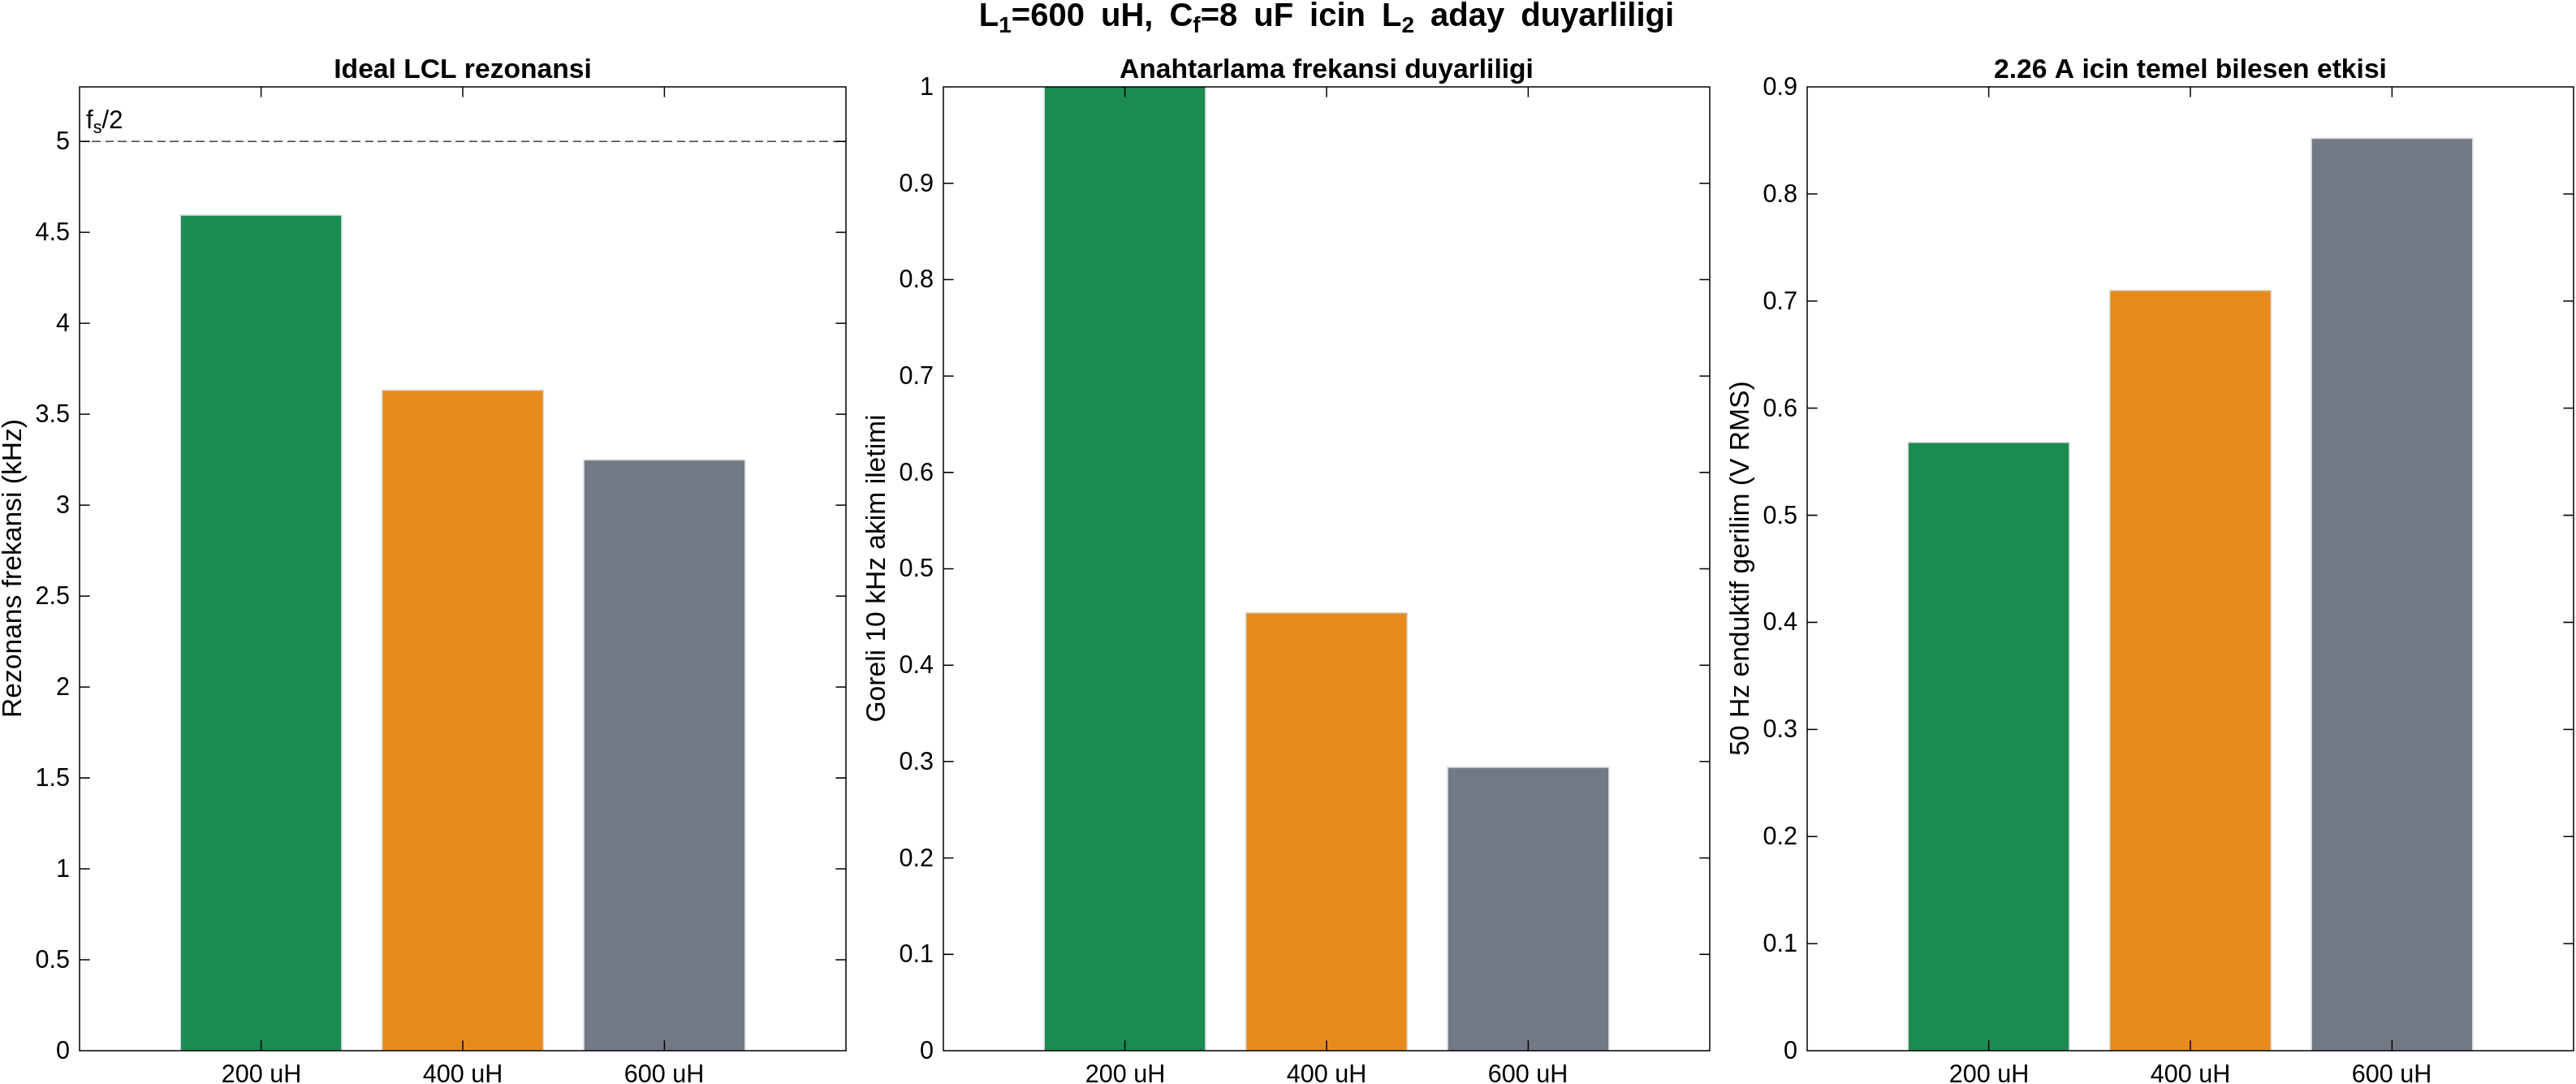
\includegraphics[width=\textwidth]{sonuclar/l2_aday_degerlendirme_20260826.png}
  \caption{$L_1=\SI{600}{\micro\henry}$ ve $C_f=\SI{8}{\micro\farad}$ için $L_2$ aday duyarlılığı: ideal rezonans frekansı, \SI{10}{\kilo\hertz} şebeke akımı iletimi ve Senaryo~1'deki \SI{2.26}{\ampere} RMS akımda \SI{50}{\hertz} toplam endüktif gerilim etkisi. Yeşil sütun nihai kaynak seçimini, turuncu eski model ayarını, gri ise faz etiketi olarak ayrıştırılan değeri göstermektedir.}
  \label{fig:l2-aday-degerlendirme}
\end{figure}

\subsection{Yarıiletken Eşlemesi ve R2025b Model Katmanları}

Gelen veri sayfaları, blok ekranları ve Senaryo~1 modelinin bağlı elemanları birlikte incelendiğinde, dört IGBT ile harici diyotların aynı ortak parametre kümesiyle temsil edilemeyeceği belirlenmiştir. Faz kolunun dış anahtarları $S_1$--$S_2$ SKM100GB12T4, iç/nötr anahtarları $S_3$--$S_4$ IXYN100N65C3H1, harici $D_1$--$D_2$ diyotları ise DSEI2x61-12B olarak eşlenmiştir. DSEI parametrelerinin IGBT'lerin iç veya ters paralel diyotlarına yayılması fiziksel olarak doğru değildir. Tablo~\ref{tab:yariiletken-esleme}, R2025b çalışma kopyasında kullanılan izlenebilir eşlemeyi vermektedir.

\begin{table}[htbp]
  \centering
  \caption{Senaryo~1 yarıiletkenlerinin parça kodu, model rolü ve R2025b çalışma kopyasındaki eşlemesi.}
  \label{tab:yariiletken-esleme}
  \footnotesize
  \begin{tabularx}{\textwidth}{>{\raggedright\arraybackslash}p{0.13\textwidth} >{\raggedright\arraybackslash}p{0.23\textwidth} >{\raggedright\arraybackslash}p{0.27\textwidth} >{\raggedright\arraybackslash}X}
    \toprule
    Devre rolü & Parça kodu & Bağlı model blokları & Uygulanan kanıt / sınır \\
    \midrule
    $S_1$--$S_2$ dış IGBT & SKM100GB12T4 & \texttt{N-Channel IGBT}, \texttt{N-Channel IGBT4} & Modeldeki SKM veri sayfasına dayalı doğrulanmış şablondan aktarıldı. \\
    $S_3$--$S_4$ iç IGBT & IXYN100N65C3H1 & \texttt{N-Channel IGBT2}, \texttt{N-Channel IGBT3} & Modeldeki IXYN veri sayfasına dayalı doğrulanmış şablondan aktarıldı. \\
    $D_1$--$D_2$ harici diyot & DSEI2x61-12B & \texttt{Diode6}, \texttt{Diode7} & $V_f=\SI{1.35}{\volt}$, $R_{\mathrm{on}}=\SI{8.5}{\milli\ohm}$ ve verilen ters toparlanma kümesi yalnız bu iki bloğa uygulandı. \\
    IGBT iç/ters paralel diyotları & Aygıta özgü & Diğer bağlı diyot blokları & DSEI ile değiştirilmedi; aygıta özgü davranış korunmalıdır. \\
    \bottomrule
  \end{tabularx}
\end{table}

Tam veri sayfası akım--gerilim ve anahtarlama kaybı tabloları, kısa süreli cihaz stresi ve kayıp teyidi için ayrıntılı model katmanını oluşturur. Kararlı hâl THD ve senaryo taraması ise aynı topoloji ve filtreyi kullanan, fakat cihaz dinamikleri sadeleştirilmiş sistem katmanında yürütülmelidir. İki katmanın sonuçları aynı kanıt olarak birleştirilmeyecek; sistem katmanındaki verim, ayrıntılı cihaz kayıplarıyla çapraz denetlenmeden nihai kabul edilmeyecektir.

\tezcalismanotu{D3-3 --- Parametrelerin kaynak dosyalarla kilitlenmesi}{$L_1$--$C_f$--$L_2$ seti kaynak ayrıştırmasıyla \SI{600}{\micro\henry}--\SI{8}{\micro\farad}--\SI{200}{\micro\henry} olarak kapatılmıştır. Tablo~\ref{tab:sistem-parametreleri} içindeki diğer `DOĞRULANACAK' alanlar kontrol kodu ve ölçüm kaydıyla doldurulacaktır. Toplam veya yarım DA bara tanımı, 20~kVA--25~kW--30~kW anma ifadeleri, anahtarlama/örnekleme frekansları, PR kazançları, gecikme ve LCL sönümleme yöntemi tek koşu yapılandırmasında tutarlı hâle gelmeden sayısal model nihai kabul edilmeyecektir.}

\section{Benzetim ve Deneysel Doğrulama Metodolojisi}

Önerilen anahtarlama ve kompanzasyon yöntemleri aynı model, çalışma noktası ve ölçüm tanımları altında karşılaştırılacaktır. Temel karşılaştırma kolları klasik tamamlayıcı anahtarlama, nötr anahtar susturma yöntemi ve Sin\textsuperscript{3} kompanzasyonlu nötr anahtar susturma yöntemi olarak belirlenmiştir. Her kol için aynı DA bara gerilimi, şebeke gerilimi, filtre, anahtarlama frekansı, örnekleme frekansı, denetleyici katsayıları ve veri işleme penceresi kullanılacaktır.

Jürinin anma gücünde kapalı çevrim çalışma talebi nedeniyle doğrulama yalnızca düşük güç noktasıyla sınırlandırılmayacaktır. Tablo~\ref{tab:dogrulama-matrisi}, düşük, orta ve anma gücü bölgelerinde karşılaştırılacak yöntemleri, kaydedilecek büyüklükleri ve raporlanacak ölçütleri aynı deney planında birleştirmektedir. Kararlı durum ölçümlerine ek olarak referans basamağı ve şebeke gerilimi değişimi gibi geçici durumların eklenmesi, verim ve THD iyileşmesinin kararlılık veya doyum pahasına elde edilip edilmediğini sınamak için gereklidir. Güvenlik veya donanım sınırları anma gücü deneyini engellerse, erişilebilen en yüksek deney noktası açıkça yazılacak ve kalan bölge doğrulanmış yüksek doğruluklu benzetim ile ayrıştırılacaktır.

\begin{table}[htbp]
  \centering
  \caption{\juriistegietiketi\ Önerilen karşılaştırmalı doğrulama matrisi.}
  \label{tab:dogrulama-matrisi}
  \small
  \begin{tabularx}{\textwidth}{p{0.19\textwidth} p{0.19\textwidth} X X}
    \toprule
    Çalışma bölgesi & Yöntemler & Kaydedilecek büyüklükler & Raporlanacak ölçütler \\
    \midrule
    Düşük güç & Klasik; susturma; susturma + Sin\textsuperscript{3} & $v_{dc}$, $v_g$, $i_1$, $i_2$, kapı işaretleri, denetleyici çıkışı & Verim, faz ve $L_1$ THD, üçüncü harmonik, ters akım alanı, RMS akım \\
    Orta güç & Aynı üç yöntem & Aynı ölçüm kanalları ve aynı işleme penceresi & Verim, THD, güç faktörü, kontrol eforu, doyum \\
    Anma gücü & En az klasik ve nihai öneri & Akım izleme, sıcaklık, DA bara dengesi, koruma ve geçici rejim & Kapalı çevrim kararlılığı, THD, verim, doyum ve güvenli çalışma \\
    Geçici rejim & Referans/güç basamağı ve gerilim değişimi & Referans, ölçülen akım, modülasyon komutu, hata/koruma işaretleri & Yerleşme süresi, aşım, akım sınırı ve yeniden toparlanma \\
    \bottomrule
  \end{tabularx}
\end{table}

\begin{center}
\juriistegietiketi\ \small Düşük, orta ve anma gücü karşılaştırması ile deneysel test talebi doğrudan test matrisine dönüştürülmüştür.
\end{center}

Karşılaştırmaların aynı tanımlarla tekrarlanabilmesi için pencere başlangıcı $t_0$ ve kararlı durum analiz süresi $T_w$ olarak tanımlansın. DA bara gerilimi ile akımı $v_{\mathrm{dc}}$ ve $i_{\mathrm{dc}}$; şebeke tarafı faz gerilimleri ile akımları $v_{g,a},v_{g,b},v_{g,c}$ ve $i_{g,a},i_{g,b},i_{g,c}$ ile gösterildiğinde ortalama DA ve üç faz AA güçleri
\begin{equation}
  \begin{aligned}
    P_{\mathrm{dc}} &= \frac{1}{T_w}\int_{t_0}^{t_0+T_w}v_{\mathrm{dc}}(t)i_{\mathrm{dc}}(t)\,\mathrm{d}t, \\
    P_{\mathrm{ac}} &= \frac{1}{T_w}\int_{t_0}^{t_0+T_w}\left[v_{g,a}(t)i_{g,a}(t)+v_{g,b}(t)i_{g,b}(t)+v_{g,c}(t)i_{g,c}(t)\right]\,\mathrm{d}t
  \end{aligned}
  \label{eq:guc-ortalama-tanimlari}
\end{equation}
olarak hesaplanacaktır. Eşitlik~\eqref{eq:guc-ortalama-tanimlari} için akım yönleri, deşarj sırasında $P_{\mathrm{dc}}>0$ ve şebekeye aktarılan güç için $P_{\mathrm{ac}}>0$ olacak biçimde seçilecektir. Deşarj yönündeki yüzde verim
\begin{equation}
  \eta=100\frac{P_{\mathrm{ac}}}{P_{\mathrm{dc}}}
  \label{eq:verim-tanimi}
\end{equation}
biçiminde raporlanacaktır. Eşitlik~\eqref{eq:verim-tanimi}, yalnızca aynı zaman penceresinden elde edilen giriş ve çıkış güçlerine uygulanacaktır. Akımın $h$'inci harmonik RMS bileşeni $I_h$, temel bileşen RMS değeri $I_1$, hesaba katılan en büyük harmonik mertebesi $H$, örnek sayısı $N_s$ ve örnek indisi $k$ ile gösterilsin. Ayrık referans ve ölçülen akım örnekleri $i^{\ast}[k]$ ile $i[k]$ olduğunda akım toplam harmonik bozunumu ve akım izleme hatası
\begin{equation}
  \begin{aligned}
    \mathrm{THD}_i &=100\frac{\sqrt{\sum_{h=2}^{H}I_h^2}}{I_1}, \\
    \mathrm{RMSE}_i&=\sqrt{\frac{1}{N_s}\sum_{k=1}^{N_s}\left(i^{\ast}[k]-i[k]\right)^2}
  \end{aligned}
  \label{eq:thd-rmse-tanimlari}
\end{equation}
ile belirlenecektir \citep{Teodorescu2011,IEC61000}. Eşitlik~\eqref{eq:thd-rmse-tanimlari} kullanılırken pencere uzunluğu, pencereleme fonksiyonu ve örnekleme frekansı her sonuçla birlikte kaydedilecektir.

Önerilen yöntemin fiziksel hedefini yalnızca THD üzerinden değerlendirmemek için referans akıma ters endüktör akımının büyüklük--zaman etkisini veren ters akım alanı $A_{\mathrm{rev}}$ ve $j$ numaralı anahtarın ikili kapı durumu $q_j[k]\in\{0,1\}$ üzerinden geçiş sayısı $N_{\mathrm{sw},j}$ tanımlansın. İşaret fonksiyonu $\operatorname{sgn}(\cdot)$ kullanılarak
\begin{equation}
  \begin{aligned}
    A_{\mathrm{rev}} &= \int_{t_0}^{t_0+T_w}\max\!\left[-i_L(t)\operatorname{sgn}\!\left(i^{\ast}(t)\right),0\right]\,\mathrm{d}t, \\
    N_{\mathrm{sw},j} &= \sum_{k=2}^{N_s}\left|q_j[k]-q_j[k-1]\right|,
    \qquad q_j[k]\in\{0,1\}
  \end{aligned}
  \label{eq:ters-akim-anahtarlama-olcutleri}
\end{equation}
Eşitlik~\eqref{eq:ters-akim-anahtarlama-olcutleri} içindeki $N_{\mathrm{sw},j}$ açma ve kapama kenarlarını ayrı geçişler olarak sayar; anahtarlama çevrimi istenirse değer uygun kenar eşleştirmesiyle ayrıca hesaplanmalıdır. Söz konusu ölçütler, verim değişiminin gerçekten ters enerji dolaşımı ve azalan anahtarlama etkinliğiyle ilişkili olup olmadığını sınamak için kullanılacaktır.

Verim hesabında DA giriş gücü ile AA çıkış gücü eşzamanlı veya zaman farkı açıkça sınırlandırılmış kayıtlar üzerinden karşılaştırılmalıdır. Eski deney altyapısında DA ve AA analizörleri arasındaki en yüksek kayıt gecikmesinin yaklaşık \SI{50}{\milli\second} olduğu, haberleşme çevriminin \SI{1}{\second} içinde tamamlandığı belirtilmiştir. Geçici rejim değerlendirmesi için söz konusu haberleşme kayıtları yeterli değildir; osiloskop veya eşzamanlı veri toplama kaydı kullanılmalıdır. THD hesabında pencere uzunluğu, temel frekans, örnekleme frekansı, harmonik üst sınırı ve analiz edilen kanal açıkça yazılacaktır.

Deneysel kanıt zinciri ham kayıt, işleme betiği veya hesap yöntemi, üretilen tablo/şekil ve tezdeki iddia arasında izlenebilir bağlantı kurmalıdır. Her sonuç şeklinin dosya adı, çalışma noktası, kullanılan yöntem, ölçüm cihazı ve tarih bilgisi bir deney kayıt tablosunda tutulacaktır. Böylece önceki tezde dağınık sunulan donanım ve ölçüm bilgileri, tekrarlanabilir bir yöntem çerçevesine dönüştürülecektir.

\tezcalismanotu{D3-4 --- Modelden tez iddiasına izlenebilirlik}{Her nihai benzetim ve deney sonucu için kaynak `.slx/.m/.mat` veya ham ölçüm dosyası, koşu kimliği, parametre özeti, işleme betiği, üretilen şekil/tablo ve desteklediği tez iddiası tek çizelgede bağlanacaktır. Önceki tezden alınan raster sonuçlar yalnız tarihsel kayıt sayılacak; aynı çalışma noktası yeniden üretilemediğinde yeni model sonucuymuş gibi kullanılmayacaktır.}

\section{Bölüm Sonucu}

Sistem mimarisi güç, ölçüm ve denetim yollarını ayıracak biçimde tanımlanmış; T-tipi faz kolunun üç gerilim seviyesi ve dört temel akım yolu ortak gösterim altında toplanmıştır. Düşük modülasyon bölgesinde senkron-buck eşdeğeri üzerinden ters akım eşiği açıklanmış, LCL filtre için durum denklemleri ve ideal aktarım fonksiyonu kurulmuştur. Sin\textsuperscript{3} terimi ana katkıyı gölgeleyen bağımsız bir kontrol stratejisi olarak değil, nötr anahtar susturma yöntemini tamamlayan ikincil kompanzasyon yolu olarak konumlandırılmıştır.

Jüri taleplerine karşılık genel blok diyagram, model katmanları tablosu, ortak tabanlı vektör çalışma modları, faz başına LCL ölçüm şeması, işlevsel denetim blok diyagramı, birleşik parametre tablosu ve düşük--orta--anma gücü doğrulama matrisi eklenmiştir. Verim, THD, izleme hatası, ters akım alanı ve anahtarlama geçiş sayısı aynı yöntem altında matematiksel olarak tanımlanmıştır. Eksik elektriksel ve denetim değerleri açıkça işaretlenmiş; sonraki adımda kaynak kod, benzetim dosyası, devre şeması ve ham deney kayıtları üzerinden doldurulacak alanlar ayrıştırılmıştır. Kurulan model, sonraki bölümlerde önerilen anahtarlama yönteminin analizi ile Sin\textsuperscript{3} kapalı çevrim/Bode incelemesine temel oluşturmaktadır.
